% Common commands
\def \logg {$\log{g}$}
\def \rsun {$R_{\sun}$}
\def \msun {$M_{\sun}$}
\def \lsun {$L_{\sun}$}
\def \rstar {$R_{\star}$}
\def \mstar {$M_{\star}$}
\def \tstar {$T_{\star}$}
\def \rp {$R_{p}$}
\def \mp {$M_{p}$}
\def \sp {$S_{p}$}
\def \teq {T$_{\rm eq}$}
\def \rj {$R_{J}$}
\def \mj {$M_{J}$}
\def \re {$R_{\earth}$}
\def \me {$M_{\earth}$}
\def \se {$S_{\earth}$}
\def \kepler {\emph{Kepler}}
\def \KEPLER {\emph{KEPLER}}
\def \keplers {\emph{Kepler's}}
\def \th {$^{\rm th}$}

% Important numbers
\def \ntces {34,032}        % Number of DR25 TCEs, includes bogus
\def \ntcesnobogus {32,534}        % Number of DR25 TCEs, no bogus
\def \npredrtwentyfourkois {7,348}  % Number of KOIS pre-DR24.
\def \npredrtwentyfivekois {8,826}  % Number of KOIs pre-DR25
\def \nkebs {2,605}         % Number of EBWG True EBs used in ephem matching.
\def \nephemmatch {1,859}   % Number of TCEs ruled as FPs due to ephemeris matching in DR24.
\def \nonlyephemmatch {106} % Number of TCEs ruled as FPs ONLY due to ephemeris matching in DR24.

\hyphenation{injTCE}  % Makes it so that "injTCE" is never hyphenated to break a line
\hyphenation{injTCEs}   % Makes it so that "injTCEs" is never hyphenated to break a line


% using aastex version 6

% \documentclass[onecolumn]{aastex6}

\documentclass[apj,twocolappendix,numberedappendix]{emulateapj}

\setcounter{secnumdepth}{4}  % Required to get section headers like  4.1.2.1 as required by AAS journal style guide

\let\underscore\_
\renewcommand{\_}{\discretionary{\underscore}{}{\underscore}}  % This and the previous line lets the mneonic flags gracefully line wrap


% These are the available options:
%   manuscript  : onecolumn, doublespace, 12pt fonts
%   preprint    : onecolumn, single space, 10pt fonts
%   preprint2   : twocolumn, single space, 10pt fonts
%   twocolumn   : a two column article. Probably not needed, but here just in case.
%   onecolumn   : a one column article; default option.
%   twocolappendix: make 2 column appendix
%   onecolappendix: make 1 column appendix is the default.
%   astrosymb   : Loads Astrosymb font and define \astrocommands.
%   tighten     : Makes baselineskip slightly smaller
%   times       : uses times font instead of the default
%   linenumbers : turn on lineno package.
%   trackchanges : required to see the revision mark up and print output
%   numberedappendix: Labels appendix sections A, B, ... This is the default.
%   appendixfloats: Needed. Resets figure and table counters to zero

%% these can be used in any combination, e.g.
%%
%% \documentclass[twocolumn,twocolappendix,linenumbers,trackchanges]{aastex6}

\usepackage{amsmath}
%% If you want to create your own macros, you can do so
%% using \newcommand. Your macros should appear before
%% the \begin{document} command.

\newcommand{\vdag}{(v)^\dagger}
\newcommand\aastex{AAS\TeX}
\newcommand\latex{La\TeX}
\newcommand\Kepler{\textit{Kepler}}
\newcommand\red{\textcolor{red}}
\newcommand\blue{\textcolor{blue}}
%% You can insert a short comment on the title page using the command below.
\slugcomment{Introductory Outline. \today}
%%
%% If you wish, you may supply running head information, although
%% this information may be modified by the editorial offices.
%%\shorttitle{\aastex sample article}

\shortauthors{Thompson et al.}




\begin{document}
%% You can add a light gray and diagonal water-mark to the first page
%% with this command:
%%\watermark{\today}

\title{Planetary Candidates Observed by \Kepler. VIII.\\
A Fully Automated Catalog Based on Quarters 1 through 17, Data Release 25\\Tuned For High Completeness and Reliability. }

%\author{Susan E. Thompson and others}
% %Authors Names Kept Separately for clarity.
% \AuthorCallLimit=20
% \fullcollaborationName{Kepler Mission Catalog Team}

\author{Susan E. Thompson\altaffilmark{0,1,2}}
%\email{susan.e.thompson@nasa.gov}
\author{Jeffrey L. Coughlin\altaffilmark{2}}
\author{Kelsey Hoffmann\altaffilmark{2}}
\author{Fergal Mullally\altaffilmark{1,2}}
\author{Christopher Burke\altaffilmark{1,2}}
\author{Jessie L. Christiansen\altaffilmark{3}}
\author{Michael Haas\altaffilmark{1}}
\author{Steve Bryson\altaffilmark{1}}
\author{Natalie Batalha\altaffilmark{1}}
\author{Joseph Catanzarite\altaffilmark{1,2}}
\author{Jason Rowe\altaffilmark{4}}
\author{Douglas Caldwell\altaffilmark{1,2}}
%\altaffiltext{0}{Susan E. Mullally, susan.e.thompson@nasa.gov}
%\altaffiltext{1}{SETI Institute, 189 Bernardo Ave, Mountain View, CA}
%\altaffiltext{2}{NASA Ames Research Center, Moffett Field, CA}
%\altaffiltext{3}{NExScI}

\author{The Rest of the Kepler Team}
%\author{Interpreters of Catalog}
%\author{Created List of TCEs}
%\author{Made Data Available}
%\author{Made mission possible}

\altaffiltext{0}{Susan E. Mullally, email: susan.e.thompson@nasa.gov}
\altaffiltext{1}{NASA Ames Research Center, Moffett Field, CA}
\altaffiltext{2}{SETI Institute, 189 Bernardo Ave, Mountain View, CA}
\altaffiltext{3}{NExScI}
\altaffiltext{4}{Someplace wonderful I'm sure. Yes.}

\begin{abstract}
Enlightening words about the purpose of this final Kepler Catalog and how it fits in with the other Kepler Planet Candidate catalogs. Then some details about how many KOIs we added and how many are planet candidates. 
Overall, the purpose of this paper is to describe how we sifted through the DR25 TCE table and identified the planet candidates, the transiting candidates with significant secondaries, background eclipsing binaries, ephemeris matches and the false alarms. It also needs to describe how we arrive at the reported physical parameters of each planet, so that interesting populations for occurrence rates and follow-up can be identified.  Finally the Completeness and Reliablity of the catalog should be discussed.


Here is a basic outline.
\begin{itemize}
\item Introduction  (Kepler is great blah, blah, KOI catalog blah blah, Cool Discoveries..)

\item A description of the Q1-Q17 DR25 TCEs

\item A description of Injection and Inversion as True Candidates and False Positives.

\item A description of the Robovetter. Summarize the Robovetter, but lean heavily on Coughlin (2016). Discuss why we needed to improve the Robovetter.  Each metric that changed from DR24 Robovetter should be discussed. A list of all minor RoboVetter flags needs to be created and how they relate to the major flags. A discussion of the Robovetter Scores and how they were calculated.

\item A discussion of how the Robovetter metrics were tuned, how were thresholds set? 

\item Evaluate the Completeness of the catalog based on transit injection in MES vs. Period. Also discuss the Confirmed planets and the number that are missed. Give a sense as to where the robovetter is missing planets.

\item Discuss the Effectiveness. Discuss the importance of reliability and how we can use Inversion to get an estimate (a bound?) of the reliability across MES and Period. Also discuss the False Positive table and the number of incorrect dispositions.  Give a sense as to where/when robovetter is ineffective and/or unreliable.

\item Creating the Catalog: Federating to old KOIs, Transit model fits and comparision to DV, how the robovetter was run (inputs/outputs, a summary),  Catalog deliverables. 

\item Analysis of the content of the catalog: Show Candidates on the radius vs. insolation flux labeled by stellar temperature (Coughlin Fig 7.), discuss Multi-planet systems, discuss new individual Rocky-HZ Planet Candidates, enumerate the number of new KOIs of different sizes.

\item Discussion of how to use this catalog to do occurrence rates. i.e. what needs to be considered (Completeness and Reliability, suspicious areas of parameter space, are additional cuts required?), not an actual calculation. Indicate what information will be delivered to NExScI to help with these calculations. 


\end{itemize}

%\textcolor{red}
%{
Items we may want to discuss in the paper but I have decided to leave out.
\begin{itemize}
\item The effectiveness or completeness of the catalog as a function of planetary radius and semi-major axis. (ie derived from fits) 
\item A specific list of confirmed planets that now have a reason to be doubted (if any exist)
\item A comparison to EB catalog
\item Analysis of the injected EBs (secondaries) in terms of effectiveness.
\item Measurement of effectiveness or completeness based on hand vetting.
\item Full analysis of completeness and reliability in terms of insolation flux and planet radius. 
\end{itemize}

Items that do not belong in this paper:
\begin{itemize}
\item An estimate of eta Earth or the occurrence rate for any type of planet.
\item Autovetter Results
\item Discussion of metrics not used by the Robovetter.
\item Complete description of the logic of the Robvetter (i.e. see Coughlin et al.)
\item A list of what was missed that are in other Kepler catalogs (Planet Hunters Catalog, Ojeda short period ones, previous KOI Tables, Confirmed planets.)
\end{itemize}
%}

\end{abstract}

\keywords{catalogs --- planetary systems --- planets and satellites: detection --- stars: statistics --- surveys --- techniques: photometric}

\section{Introduction}

%One of the goals of NASA's astrophysics missions is to understand the Earth's place in the Universe.
\Kepler{'s} mission to measure the frequency of Earth-size planets in the Galaxy is an important step towards understanding the Earth's place in the Universe.  Launched in 2009, the \Kepler{} Mission \citep{Koch2010,Borucki2016} stared almost continuously at a single field for four years (or 17, $\approx$90~day quarters), recording the brightness of $\approx$200,000 stars ($\approx$160,000 stars at a time) at a cadence of 29.4 minutes over the course of the mission. \Kepler{} detected transiting planets by observing the periodic decrease in the observed brightness of a star when an orbiting planet crossed the line of sight from the telescope to the star. \Kepler{'s} prime-mission observations concluded in 2013 when it lost a second of four reaction wheels, three of which were required to maintain the stable pointing.  From the ashes of \Kepler{} rose the \Ktwo{} mission which continues to find exoplanets in addition to a whole host of astrophysics enabled by its observations of fields in the ecliptic \citep{Howell2014,VanCleve2016K2}. 
While not the first to obtain high-precision, long-baseline photometry to look for transiting exoplanets \citep[see e.g.,][]{Barge2008,ODonovan2006}, \Kepler{} and its plethora of planet candidates revolutionized exoplanet science. The large number of Kepler planet detections from the same telescope opened the door for occurrence rate studies and has enabled some of the first measurements of the frequency of planets similar to the Earth in our Galaxy.  To further enable those types of studies, we present here the planet catalog that resulted from the final search of the original \Kepler{} mission data along with the tools provided to understand the biases inherent in the search and vetting done to create that catalog.
%In this paper we use the original four years of Kepler data to create a fully automated catalog designed to enable planetary occurrence rates, even for terrestrial-size planets in one-year orbits.

First, we put this work in context by reviewing some of the scientific achievements accomplished using \Kepler{} data.  Prior to \Kepler{,} most exoplanets were discovered by radial velocity methods \citep[e.g.][]{Mayor1995}, which largely resulted in the detection of Neptune- to Jupiter-mass planets in orbital periods of days to months. The high precision photometry and the four-year baseline of the \Kepler{} data extended the landscape of known exoplanets.  To highlight a few examples, \citet{Barclay2013} found evidence for a moon-size terrestrial planet in a 13.3 day period orbit, \citet{Quintana2014} found evidence of an Earth-size exoplanet in the habitable zone of the M dwarf Kepler-186, and \citet{Jenkins2015} statistically validated a super-Earth in the habitable zone of a G-dwarf star. Additionally, for several massive planets \Kepler{} data has enabled measurements of planetary mass and atmospheric properties by using the photometric variability along the entire orbit \citep{Shporer2011,Mazeh2012,Shporer2017}. \Kepler\ data has also revealed hundreds of compact, co-planar, multi-planet systems, e.g., the six planets around Kepler-11 \citep{Lissauer2011}, which collectively have told us a great deal about the architecture of planetary systems \citep{Lissauer2011b,Fabrycky2014}.   Exoplanets have even been found orbiting binary stars, e.g., Kepler-16~(AB)~b \citep{Doyle2011}.

Other authors have taken advantage of the long time series, near-continuous data set of 206,150\footnote{This tally only includes the targeted stars and not those observed by ``accident'' in the larger apertures.} stars to advance our understanding of stellar physics through the use of asteroseismology. Of particular interest to this catalog is the improvement in the determination of stellar radius \citep[e.g.,][]{Huber2014a,Mathur2017ApJS} which can be one of the most important sources of error when calculating planetary radii. \Kepler{} data was also used to track the evoluation of star-spots created from magnetic activity and thus enabled the measurement of stellar rotation rates \citep[e.g.][]{Aigrain2015,Garcia2014,McQuillan2014,Zimmerman2017}. Studying stars in clusters enabled \citet{Meibom2011} to map out the evolution of stellar rotation as stars age. \Kepler{} also produced light curves of 2876\footnote{This represents the number reported in the Kepler Binary Catalog, \url{http://keplerebs.villanova.edu}, in August 2017.} eclipsing binary stars \citep{Prsa2011,Kirk2016} including unusual binary systems, such as the eccentric, tidally-distorted, Heartbeat stars \citep{Welsh2011,Thompson2012,Shporer2016hb} that have opened the doors to understanding the impact of tidal forces on stellar pulsations and evolution \citep[e.g.,][]{Hambleton2017,Fuller2017}.

The wealth of astrophysics, and the size of the \Kepler{} community, is in part due to the rapid release of \Kepler{} data to the NASA Archives: the Exoplanet Archive \citep[][]{Akeson2013} and the MAST (Mikulski Archives for Space Telescopes).  The \Kepler{} mission released data from every step of the processing \citep{Thompson2016KAM,Stumpe2014,Bryson2010b}, including the results of its planet searches. The results of both the original searches for periodic signals (known as the TCEs or Threshold Crossing Events) and the well-vetted KOIs (Kepler Objects of Interest) were made available for the community.  The combined list of \Kepler{'s} planet candidates found from all searches can be found in the cumulative KOI table\footnote{\url{https://exoplanetarchive.ipac.caltech.edu/cgi-bin/ TblView/nph-tblView?app=ExoTbls\&config=cumulative}}.  The KOI table we present here is from a single search of the DR25 light curves. While the search does not include new observations, it was performed using an improved version of the \Kepler{} Pipeline \citep[version 9.3,][]{Jenkins2017}. For a high-level summary of the changes to the Pipeline, see the DR25 data release notes \citep{DRN25,KDCH}. The \Kepler{} Pipeline has undergone successive improvements since launch as the data characteristics have become better understood.

%The \Kepler{} mission released data from every step of the processing, including unprocessed images, systematic-error-corrected light curves \citep{Stumpe2014}, lists of planet candidates, as well as ancillary data such as pixel response functions \citep{Bryson2010b}.
%This table is actually the combination of individual KOI tables that resulted from searches with progressively longer baselines \citep{Borucki2011a, Batalha2013, Burke2014, Rowe2015cat, Mullally2015cat,Coughlin2016}.
%The light curves used for the planet search discussed here are all part of Data Release 25 (DR25) and are described in detail in \citet{DRN25} and \citet{KDCH}.The mission cataloged the results of many of its searches for periodic transit signals in the data. 

%{\color{blue}
The photometric noise at time scales of the transit is what limits \Kepler{} from finding small terrestrial-size planets. Investigations of the noise properties of \Kepler{} exoplanet hosts by \citet{Howell2016} showed that those exoplanets with the radii $\leq$1.2\re{} are only found around the brightest, most photometrically quiet stars. As a result, the search for the truly Earth-size planets are limited to a small subset of \Kepler{'s} stellar sample.  Analyses by \citet{Gilliland2011,Gilliland2015} show that the primary source of the observed noise was indeed inherent to the stars, with a smaller contributions coming from imperfections in the instruments and software. Unfortunately, the typical noise level for 12$^{th}$ magnitude solar-type stars is closer to 30\,ppm \citep{Gilliland2015} than the 20\,ppm expected from \citet{Jenkins2002a}, causing \Kepler{} to need a longer baseline to find a significant number of Earth-like planets around Sun-like stars.   Ultimately, this higher noise level impacts \Kepler{'s} planet yield. And, because different stars have different levels of noise, the transit depth to which the search is sensitive varies across the sample of stars. This bias must be accounted for when calculating occurrence rates, and is explored in-depth for this run of the \Kepler{} Pipeline by the transit injection and recovery studies of \citet[][]{Burke2017b,Burke2017a,Christiansen2017}.
%}
 

%%This might be a good place for a paragraph regarding follow-up observing.
%{\color{blue}
To confirm the validity and further characterize identified planet candidates, the \Kepler{} mission benefited from an active, funded, follow-up observing program. This program used ground-based radial velocity measurements to determine the mass of exoplanets \citep[e.g.,][]{Marcy2014} when possible and also ruled out other astrophysical phenomena, like background eclipsing binaries, that can mimic a transit signal.  The follow-up program obtained high-resolution imaging of $\approx$90\% of known KOIs \citep[e.g.,][]{Furlan2017} to identify close companions (bound or unbound) that would be included in \Kepler{'s} rather large 3.98\,$\arcsec$ pixels.  The extra light from these companions must be accounted for when determining the depth of the transit and the radii of the exoplanet.  While the \Kepler{} Pipeline accounts for the stray light from stars in the Kepler Input Catalog (\citealt{Brown2011}; and see flux fraction in \S2.3.1.2 of the Kepler Archive Manual; \citealt{Thompson2016KAM}), the sources identified by these high-resolution imaging catalogs were not included. Based on the analysis by \citet{Ciardi2015}, where they considered the effects of multiplicity, planet radii are underestimated by a factor averaging\,$\simeq$1.5 for G dwarfs prior to vetting, or averaging $\simeq$1.2 for KOIs that have been vetted with high-resolution imaging and Doppler spectroscopy.  The effect of unrecognized dilution decreases for planets orbiting the K and M dwarfs, because they have a smaller range of possible stellar companions
%}

%Eclipsing binary systems often mimic the signal of a transit and must be weeded out through either additional confirming data \citep[such as radial velocities, e.g.][]{Marcy2014}, or statistical analysis.

Even with rigorous vetting and follow-up observations, most planet candidates in the KOI catalogs cannot be directly confirmed as planetary. The stars are too dim and the planets are too small to be able to measure a radial velocity signature for the planet.   Statistical methods study the likelihood that the observed transit could be caused by other astrophysical scenarios and have succeeded in validating thousands of \Kepler{} planets \citep[e.g.][]{Lissauer2014,Morton2016,Rowe2014,Torres2015}.  

The Q1--Q16 KOI catalog \citep{Mullally2015cat} was the first with a long enough baseline to be significantly impacted by the long-period false positives created by the instrument itself.  In that catalog (and again in this one), the majority of long-period, low SNR TCEs are ascribed to instrumental effects incompletely removed from the data before the TCE search. \Kepler\ has a variety of short timescale (on the order of a day or less), non-Gaussian noise sources including focus changes due to thermal variations, signals imprinted on the data by the detector electronics, noise caused by solar flares, and the pixel sensitivity changing after the impact of a high energy particle (known as a sudden pixel sensitivity drop-out, or SPSD). Because the large number of TCEs associated with these types of errors, and because the catalog was generated to be intentionally inclusive (i.e. high completeness), many of the long-period candidates in the Q1--Q16 KOI catalog are expected to simply be noise.  We were faced with a similar problem for the DR25 catalog and spent considerable effort writing software to identify these types of false positives, and for the first time we include an estimate for how often these signals contaminate the catalog.

The planet candidates found in \Kepler{} data have been used extensively to understand the frequency of different types of planets in the Galaxy. Many studies have shown that small planets ($<4$\re) in short period orbits are common, with occurrence rates steadily increasing with decreasing radii \citep{Burke2016,Howard2012,Petigura2013b,Youdin2011}.  \citet{Dressing2013,Dressing2015}, using their own search, confined their analysis to M dwarfs and orbital periods less than 50\,d and determined that multi-planet systems are common around these low mass stars.  Therefore planets are more common than stars in the Galaxy (due, in part, to the fact that low mass stars are the most common stellar type). 
\citet{Fulton2017}, using improved measurements of the stellar properties \citep{Petigura2017}, looked at small planets with periods of less than 100\,d and showed that there is a valley in the occurrence of planets near 1.75\re{}. This result improved upon the results of \citet{Howard2012} and \citet{Lundkvist2016} and further verified the evaporation valley predicted by \citet{Owen2013} and \citet{Lopez2013} for close-in planets.

Less is known about the occurrence of planets in longer period orbits. Using planet candidates discovered with \Kepler{}, several papers have measured the frequency of small planets in the habitable zone of sun-like stars \citep[see e.g.][]{Burke2015,ForemanMackey16,Petigura2013b} using various methods. \citet{Burke2015} used the Q1--Q16  KOI catalog \citep{Mullally2015cat} and looked at G and K stars and concluded that 10\% (with an allowed range of 1--200\%) of solar-type stars host planets with radii and orbital periods within 20\% of that of the Earth. \citet{Burke2015} considered various systematic effects and showed that they dominate the uncertainties and concluded that improved measurements of the stellar properties, the detection efficiency of the search, and the reliability of the catalog will have the most impact in narrowing the uncertainties in such studies. 


\subsection{Design Philosophy of the DR25 catalog}

The DR25 KOI catalog is designed to support rigorous occurrence rate studies. To do that well, it was critical that we not only identify the exoplanet transit signals in the data but also measure the catalog reliability (the fraction of transiting candidates that are not caused by noise), and the completeness of the catalog (the fraction of true transiting planets detected).

The measurement of the catalog completeness has been split into two parts: the completeness of the TCE list (the transit search performed by the \Kepler\ Pipeline) and the completeness of the KOI catalog (the vetting of the TCEs). The completeness of the \Kepler\ Pipeline and its search for transits has been studied by injecting transit signals into the pixels and examining what fraction are found by the \Kepler{} Pipeline \citep{Christiansen2017, Christiansen2015b,Christiansen2013a}. \citet{Burke2015} applied the appropriate detection efficiency contours \citep{Christiansen2015} to the 50--300\,d period planet candidates in the Q1--Q16 KOI catalog \citep{Mullally2015cat} in order to measure the occurrence rates of small planets. However, that study was not able to account for those transit signals correctly identified by the \Kepler{} Pipeline but thrown-out by the vetting process. Along with the DR25 KOI catalog, we provide a measure of the completeness of the DR25 vetting process. 

\Kepler{} light curves contain variability that is not due to planet transits or eclipsing binaries. While the reliability of \Kepler\ catalogs against astrophysical false positives is mostly understood \citep[see e.g.][]{Morton2016}, the reliability against false alarms (a term used in this paper to indicate TCEs caused by intrinsic stellar variability, over-contact binaries, or instrumental noise, i.e., anything that does not look transit-like) has not previously been measured. Instrumental noise, statistical fluctuations, poor detrending, and/or stellar variability can conspire to produce a signal that looks similar to a planet transit. When examining the smallest exoplanets in the longest orbital periods, \citet{Burke2015} demonstrated the importance of understanding the reliability of the catalog, showing that the occurrence of small, earth-like-period planets around G dwarf stars changed by a factor of $\approx$10 depending on the reliability of a few planet candidates.  In this catalog we measure the reliability of the reported planet candidates against this instrumental and stellar noise.  

The completeness of the vetting process is measured by vetting thousands of injected transits found by the \Kepler{} Pipeline. Catalog reliability is measured by vetting signals found in scrambled and inverted \Kepler{} light curves and counting the fraction of simulated false alarms that are dispositioned as planet candidates. This desire to vet both the real and simulated TCEs in a reproducible and consistent manner demands an entirely automated method for vetting the TCEs.  

Automated vetting was introduced in the Q1--Q16 KOI catalog \citep{Mullally2015cat} with the Centroid Robovetter and was then extended to all aspects of the vetting process for the DR24 KOI catalog \citep{Coughlin2016}. Because of this automation, the DR24 catalog was the first with a measure of completeness that extended to all parts of the search, from pixels to planet candidates.  Now, with the DR25 KOI catalog and simulated false alarms, we also provide a measure of how effective the vetting techniques are at identifying noise signals and translate that into a measure of the catalog reliability. As a result, the DR25 KOI catalog is the first to explicitly balance the gains in completeness against the loss of reliability, instead of always erring on the side of high completeness. 

%Subsection on the abbreviations
%%List Acronyms Here
\subsection{Terms and Abbreviations}
\label{abbrev}
We try to avoid unnecessary acronyms and abbreviations, but are a few are required to efficiently discuss this catalog.  Here we itemize those terms and abbreviations that are repeatedly used in this paper:

\begin{itemize}
%\item[] \textbf{KOI}: Kepler Object of Interest. A particular ephemeris on an object that was given a KOI number. The intent is to create KOIs out of all identified events that could possibly be planet candidates or eclipsing binaries.  
\item[] \textbf{TCE}: Threshold Crossing Event identified by the Kepler Pipeline and reported in \citet{Twicken2016}.
\item[] \textbf{OBS-TCE}: Observed TCEs. TCEs found by searching the observed data, i.e. the DR25, Q1--Q17 data set.
\item[] \textbf{INJ-TCE}: Injected TCE. TCEs found that matches a known, injected transit signal.
\item[] \textbf{INV-TCE}: Inverted TCE. TCEs found when searching the inverted data set in order to simulate instrumental false alarms.
\item[] \textbf{SCR-TCE}: Scrambled TCE. TCEs found when searching the scrambled data set in order to simulate instrumental false alarms.
\item[] \textbf{KOI}: Kepler Object of Interest. Periodic events identified on a particular star that possibly have the shape of a transit or eclipse are added to the KOI table at NExScI. 
\item[] \textbf{PC}: Planet Candidate. A TCE that passed all of the Robovetter tests and metrics.
\item[] \textbf{FP}: False Positive. A TCE that failed one or many of the Robovetter tests and metrics.
\item[] \textbf{MES}: Multiple Event Statistic. A statistic that measures the significance of the observed transits in the TPS detrended, whitened light curve, see \citep{Jenkins2002a}.
\item[] \textbf{DV}: Data Validation. The module of the \Kepler\ pipeline which characterizes the transits. This module evaluates each TCE and provides a detrended light curves on which other metrics are based.
\item[] \textbf{ALT}: Alternate. An alternate detrending, based on the methods of \citet{Garcia2010}, are utilized by several metrics discussed in this paper.

\end{itemize}


\subsection{Summary and Outline of the Paper}

The DR25 KOI catalog is a uniformly-vetted list of planet candidates and false positives found by searching the DR25 \Kepler\ light curves and includes a measure of the catalog completeness and reliability. In the brief outline that follows we highlight how the catalog was assembled, how we measure the completeness and reliability, and discuss those aspects of the process that are different from the DR24 KOI catalog \citep{Coughlin2016}.

In \S\ref{s:tces} we describe the observed TCEs (\opstce s) which are the periodic signals found in the actual \Kepler\ light curves. For reference, we also compare them to the DR24 TCEs. To create the simulated data sets necessary to measure the vetting completeness and the catalog reliability, we ran the \Kepler\ Pipeline on light curves that either contained injected transits, were inverted, or were scrambled. This creates \injtce s, \invtce s, and \scrtce s, respectively (see \S\ref{s:simulated}).  

We then created and tuned a Robovetter to vet all the different sets of TCEs. \S\ref{s:robovetter} describes the metrics and the logic used to disposition TCEs into PCs and FPs.  Because the DR25 \opstce\ population was significantly different than the DR24 \opstce{s}, we developed new metrics to separate the PCs from the FPs (see Appendix \ref{s:metrics} for the details on how each metric operates.) Several new metrics examine the individual transits for evidence of instrumental noise (see \S\ref{s:indivtrans}.) As in the DR24~KOI catalog, we group FPs into four categories (\S\ref{s:majorflags}) and provide minor false positive flags (Appendix \ref{s:minorflags}) to indicate why the Robovetter decided to pass or fail a TCE.  New to this catalog is the addition of a disposition score (\S\ref{s:scores}) that gives users a measure of the Robovetter's confidence in each disposition. 


Unlike previous catalogs, for the DR25 KOI catalog the choice of planet candidate versus false positive is no longer based on the philosophy of ``innocent until proven guilty''. We accept certain amounts of collateral damage (i.e., exoplanets dispositioned as FP) in order to achieve a catalog that is uniformly vetted and has acceptable levels of both completeness and reliability, especially for the long period and low signal-to-noise PCs. In \S\ref{s:optimize} we discuss how we tuned the Robovetter using the simulated TCEs as populations of true planet candidates and true false alarms. We provide the Robovetter source code and all the Robovetter metrics for all of the sets of TCEs (\opstces, \injtces, \invtces, and \scrtces) to enable users to create a catalog tuned for other regions of parameter space if their scientific goals require it. 

We assemble the catalog (\S\ref{s:assemble}) by federating to previously known KOIs before creating new KOIs. Then to provide planet parameters, each KOI is fit with a transit model which uses a Markov Chain Monte Carlo (MCMC) algorithm to provide error estimates for each fitted parameter (\S\ref{s:mcmc}). In \S\ref{s:summary} we summarize the catalog and discuss the performance of the vetting using the \injtce, \invtce, and \scrtce\ sets. We show that both decrease significantly with decreasing number of transits and decreasing signal-to-noise.  We then discuss how one may use the disposition scores to identify the highest quality candidates, especially at long periods (\S\ref{s:crscores}.)  We conclude that not all declared planet candidates in our catalog are actually astrophysical transits, but we can measure what fraction are caused by stellar and instrumental noise. Because of the interest in terrestrial, temperate planets, we examine the high quality, small candidates in the habitable zone in \S\ref{s:hz}. Finally, in \S\ref{s:occurates} we give an overview of what must be considered when using this catalog to measure accurate exoplanet occurrence rates, including what information is available in other \Kepler{} products to do this work. 





\section{The Q1--Q17 DR25 TCEs}
\label{tcesec}
\subsection{Observed TCEs}

\label{s:tces}
As with the previous three Kepler planet candidate catalogs \citep{Coughlin2016,Mullally2015cat,Rowe2015cat}, the population of events that were used to create KOIs and planet candidates are known as Threshold Crossing Events or \opstce s.  These are periodic reductions of flux in the light curve that were found by the Transit Planet Search (TPS) module and evaluated by the Data Validation (DV) module of the Kepler Pipeline \citep{JenkinsKDPH}.   The Data Release 25 \opstce s were created by running the SOC 9.3 version of the Pipeline on the DR25, Q1--Q17 \Kepler\ PDC time-series.  For a thorough analysis of the DR25 TCEs and on the pipeline's search see \citet{Twicken2016}.  

The DR25 \opstce s, their ephemerides, and the metrics calculated by the pipeline are available at the NASA Exoplanet Archive \citep{Akeson2013}.  In this paper we endeavor to disposition these signals into planet candidates and false positives.  Because the \opstce s act as the input to our catalog, we first describe some of their properties as a whole and reflect on how they are different than the previous \Kepler\ TCE table.

We have plotted the distribution of the \ntcesnorogue\ \opstce s in terms of period in Figure~\ref{f:tces}. Notice, an excessive number of short and long period \opstce s with the number increasing with decreasing MES. 

As with previous catalogs, the short period ($<10$\,d) excess is dominated by true, sinusoidal variability of the star. The long period excess is dominated by instrumental noise. For example, a decrease in flux following a cosmic ray hit (a.k.a. SPSD, Sudden Pixel Sensitivity Drop-out), can match-up with natural fluctuations in the data to produce a TCE. Also, image artifacts known as rolling-band is very strong on some channels \citep[see \S6.7 of][]{KIH}  and since the spacecraft rolls every $\approx$90\,days, causing a star to roll onto a \Kepler\ channel with significant rolling band, these variations can easily line-up to produce TCEs at 372\,d. This is the reason for the spike in the \opstce\ population seen in Figure~\ref{f:tces}. Generally, the excess of long period TCEs is significantly larger than it was in the DR24 TCE catalog \citep{Seader2015}. Most likely, this is because DR24 implemented an aggressive and irregular veto known as the bootstrap metric \citep{JenkinsBootstrap}.  For DR25 this metric was calculated, but was not used as a veto. Also other vetoes were made less strict causing more TCEs across all periods to be created. 

To summarize, for DR25 the number of false signals among the \opstce s  is drastically larger than in any previous catalog. As a result, we expect the \opstce\ list to contain more true exoplanets than before. However, the reliability of the \opstce\ catalog is lower than it has been in the past.   

\begin{figure*}[h!]
 \begin{center}
  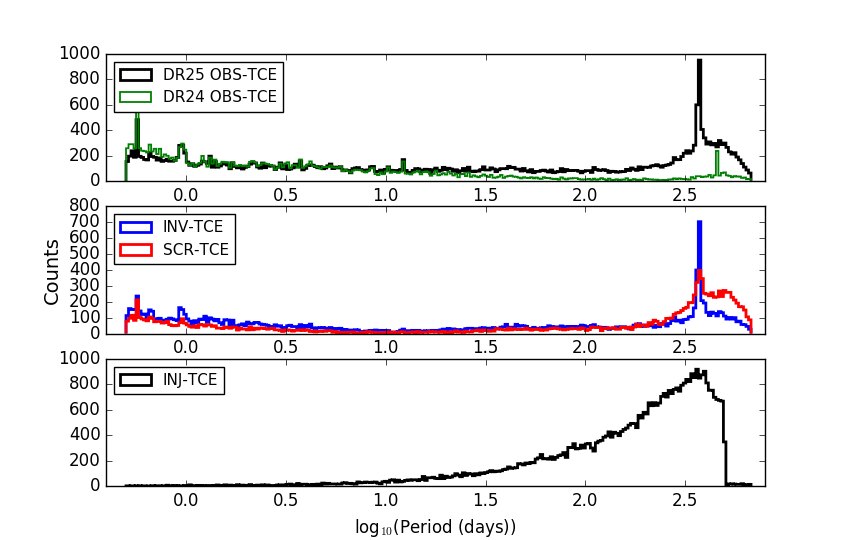
\includegraphics[width=1.0\linewidth]{fig-tcePeriods.png}
  \caption{Histogram of the log$_{10}$(period) in days of the four different TCE populations (\opstce (top, black),\scrtce (middle, red), \invtce\ (middle, blue) and \injtce (bottom, black)) used to create the DR25 catalog. In the top plot the DR24 OBS-TCE population is shown for reference.}
  %\caption{\ref{f:tces} A two dimensional histogram of the number of TCEs by log(period) and log(MES). The marginalized distributions for log(period) and log(MES) are projected along their respective axes and shown on the top and right respectively. }
  \label{f:tces} 
 \end{center}
 \end{figure*}



\subsection{Rogue TCEs}
The DR25 TCE table at NExScI contains \ntces\ DR25 Observed TCEs (\opstce s), however, in this paper we disposition \ntcesnorogue\ of these \opstce s. The remaining \opstce s are known as ``rogue" TCEs, and were created because of a bug in the Kepler pipeline which let through certain three-transit events. Because the primary purpose of this catalog is to be able to accurately calculate occurrence rates and because this same bug was not present when characterizing the completeness of the \Kepler\ Pipeline \citep{}BURKE PRODUCT REFERENCE, we ignore the rogue TCEs here. For more information see XX CITE SOMEONE HEREXX. 
Also note that all of the TCE populations (INJ, INV, SCR and OPS, see the next section) had rogue TCEs. The creation and analysis of this KOI catalog only rely on the non-rogue TCEs.




\section{Tools for Evaluating Performance}

\section{Simulated TCEs for Completeness and Reliability}
\label{s:simulated}
Because we needed a way to identify when the Robovetter was not performing well, and because we wanted to be able to measure the performance of the Robovetter, we created simulated transits and simulated false alarms. The simulated transits are created by the injecting transit signals onto the pixels of our original data.  The simulated false alarms caused by instrumental and stellar noise were created in two ways, 1) by inverting our light curve and 2) by scrambling the time order of the time series.  


\subsection{True Transits -- Injection}
\label{injectsec}
The pixel-level transit injection is similar to that used by DR24 \citep{Christiansen2016} and is described in detail for DR25 in \citep{Christiansen2017}. The pixel-level injection study provides several types of injections: those on the target star, those offset from the location of the target star, two injections on the same star to emulate an eclipsing binary, and a special period range for the M-dwarf stars.  For our purposes in this paper, we will focus on the on-target injections of all type.  These injected signals were placed on the calibrated pixel data and sent through the same \Kepler{} pipeline as the \opstce s.


\subsection{False Alarms -- Inverted and Scrambled} 

To create false alarms, the simplest thing to do was to take the normalized light curve in the transit planet search module of the \Kepler\ pipeline and multiply it by $-1$.  This flips the light curve upside down before it is whitened and searched for exoplanets.  Because the pipeline is only looking for transit-like dips in the light curve, the exoplanet transits will no longer be found. However, periodic instrumental and stellar noise will still be found.  This approach assumes that these sources of false alarms are symmetric. The period distribution of these \invtce s are shown in Figure~\ref{f:tces} as the blue histogram.  The distribution across period of these events basically emulates those seen in the \opstce s; however there are only about 60 per cent as many.  The one-year spike is clearly seen, but again is not as tall we might expect given the size of the one-year spike in the \opstce\ period distribution. 

Another method to create false alarm is to scramble the data.  The trick is to scramble the data enough to lose the coherence for the binary stars and the exoplanets in the data, but keep some of the coherency of the red noise that plagues the \Kepler\ data set.  We accomplished this by scrambling the data by year. In other words we moved year 4 to the front, followed by year 3, then 2, then 1. Q17 was kept at the end of the time series. Within each year, the order of the data did not change. The final order of the quarters in the scrambled data set was 13,14,15,16,9,10,11,12,5,6,7,8,1,2,3,4,17.  Notice that in this configuration each quarter remains in the correct \Kepler\ season (NEED TO EXPLAIN SEASON??), as so some of the yearly, rolling-band issues were detected in this way.



In Figure~\ref{f:false} we show an example of the folded light curves of an \opstce, \invtce, and \scrtce\ where the number of identified transit events is three.  Notice that for low signal-to-noise \Kepler\ data is capable of having three events due to noise line-up and produce something that looks very similar to an exoplanet transit.  

\subsubsection{Cleaning Inversion and Scrambling}
As described in \S\ref{s:reliability}, we want to use the \invtce\ and \scrtce\ sets to measure the reliability of the DR25 catalog against instrumental and stellar noise.  In order to do that well, we need to remove signals found in these sets that are not typical of those in our \opstce\ set.  For inversion there are astrophysical events that look similar to an inverted eclipse, for example the self-lensing binary star, K03278.01 \citep{Kruse2014}, and Heartbeat Binaries \citep{Thompson2012}.  With the assistance of published systems and early runs of the Robovetter, we identified any \invtce\ that could be identified as possibly one of these types of astrophysical events; 54 systems were identified in total.  Also, the shoulders of inverted eclipsing binary stars and high signal-to-noise KOIs were found by the pipeline but are not the type of false alarm we were trying to reproduce.  To summarize, we remove any \invtce\ that was found on a star that had 1) one of the identified astrophysical events, 2) detached eclipsing binaries from \citet{Kirk2016} (morphology values larger than 0.6), and 3) a known KOI with a period less than 100\,d and MES larger than 9.  The result is \ninvtces\ \invtce s and their distribution is plotted in Figure~\ref{f:tces}.

For season scrambling, we do not have to worry about the astrophysical events that emulate an inverted transit, but we do have to worry about triggering on true transits. For this reason we removed from the \scrtce\ population any one that landed on a star with a known eclipsing binary \citep{Kirk2016}, or on a previously identified KOI \citep{Coughlin2016}.  The result is \nscrtces\ \scrtce.and their distribution is plotted in Figure~\ref{f:tces}. 

After cleaning the \invtce s and \scrtce s of the eclipsing binary and KOI systems, the number of \scrtce s at periods longer than 200\,d closely matches the size and shape of the same period range in the \opstce s, except for the one-year spike.  The one-year spike is well represented by the \invtce s.  Combining the two sets appears to give us a good handle on the type and relative frequency of false alarms present in our \opstce\ population. Table\,\ref{tab:invscr} lists those \invtce s and \sctce s that we used when calculating the effectiveness and thus reliability of the catalog.

\subsection{How good are the simulated data sets}
We should show some evidence that the fraction of false alarms in the simulated data sets matches those in the actual OBS data.  Can we show that the fraction of fails by LPP, individual transits and sig-pri/Fred are approximately the same between the two sets.  Or how different are they.  Do this for low mes,


\subsection{Other Simulated sets}
We also simulated other types of false positives through transit injection \citep{Christiansen2017}. A portion of the injections were injected off the target by less than a pixel.  This is a way of testing our ability to find background eclipsing binaries by looking for small shifts in the location of the transit compared to the location of the target star.  Also, we injected two transits on some stars to emulate an eclipsing binary and test our tools to identify the presence of a significant secondary eclipse.  However because the majority of our false positives are caused by instrumental noise, and because the size of the astrophysical false positive reliability has been well characterized for \Kepler\ \citep[e.g.][]{Morton2016}, we limit our reliability discussion to those caused by instrumental and stellar noise. 


All of the data sets described above are available in their entirety at the NASA Exoplanet Archive.  All of the metrics described in \S\ref{s:robovetter} to evaluate the disposition of these TCEs are also available in the same table. 



\section{Vetting Methods and Metrics}
In the first five \Kepler{} planet candidate catalogs \citep{Borucki2011a,Borucki2011b,Batalha2013,Burke2014,Rowe2015a}, various plots and diagnostics for each TCE were visually examined by members of the Threshold Crossing Event Review Team (TCERT), which consists of professional scientists who have a thorough understanding of \kepler{} data systematics and the various types of false positive scenarios. In the sixth catalog, \citet{Mullally2015cat} employed partial automation through the use of three simple parameter cuts, principally to cull out a large number of long-period false positives, as well as a robotic procedure to identify a particular subset of centroid offsets \citep[see \S5.2 of][]{Mullally2015cat}. In the seventh catalog, \citet{Coughlin2016} fully automated the dispositioning of TCEs, a long-standing objective of the \kepler{} mission in order to enable the accurate computation of planet occurence rates.


% TALK ABOUT THE vDR24 ROBOVETTER RESULTS??
% \subsubsection{Using the DR24 Robovetter}
%  We applied the DR24 robovetter to the DR25 TCEs. 
%  We found that we needed to do better in the following areas.
%  Don't forget to cite \citet{Tange2011a}.
%  %Words about applying the DR24 robovetter to the DR25 TCEs.
Our first attempt at vetting the DR25 TCE list was done by applying the DR24 Robovetter \citep{Coughlin2016}. To do this, we calculated the metrics described in \citet{Coughlin2016}, such as the LPP Metric, the Marshall Metric, the Model-Shift Uniqueness Test, the Significant Secondary Test, the Centroid Offset and the Ephemeris matching.  We were then able to evaluate the performance of this version of the 
robovetter using the pixel-level transit injection and inversion data. 


Clearly, these results indicate that the TCE population had changed enough to require improvements to the robovetter in order to achieve a highly complete and highly reliability catalog.




% OLD TEXT JUST SAVING FOR NOW
% which requires that every TCE be dispositioned in a uniform manner so that it can be subjected to quantitative evaluation. 
%
% As manual inspection by TCERT members is very time-consuming, it is often not feasible to examine each of the $\sim$20,000 TCEs produced by the \kepler{} pipeline. While TCERT members are well-trained, as humans they do not always agree with each other, and individuals may disposition a given TCE differently depending on external factors such as the time of day, their mood, other TCEs examined recently, etc. However, humans are naturally adept at pattern recognition and categorization, and TCERT has developed an efficient and comprehensible workflow procedure, based on understood physical processes, while working on the previous six planet candidate catalogs. 
%
% Thus, for automating the TCE dispositioning process, we have specifically chosen a robotic vetting procedure that operates via a series of simple decision trees. Hereafter referred to as the ``robovetter'', it attempts to mimic the well-known human vetting process, providing a specific reason for dispositioning any TCE as a false positive. The robovetter was initially developed based on the results of the Q1--Q16 catalog \citep{Mullally2015cat} and then further refined based on the results of manual checks on the the Q1--Q17~DR24 dataset by TCERT members.


Similar to \citet{Rowe2015a}, \citep{Mullally2015cat}, and \citet{Coughlin2016}, we assign FP TCEs to one or more of the following false positive categories:


\begin{itemize}
  \item ``Not Transit-Like'': a TCE whose light curve is not consistent with that of a transiting planet or eclipsing binary, such as instrumental artifacts and non-eclipsing variable stars.
  \item ``Stellar Eclipse'': a TCE that is observed to have a significant secondary event, transit shape, or out-of-eclipse variability that indicates the transit-like event is most likely caused by an eclipsing binary. (Self-luminous, hot Jupiters with a visible secondary eclipse are also in this category, but are still given a disposition of PC.)
  \item ``Centroid Offset'': a TCE whose signal is observed to originate on a nearby star, rather than the target star, based on examination of the pixel-level data.
  \item ``Ephemeris Match Indicates Contamination'': a TCE that has the same period and epoch as another object, and is not the true source of the signal given the relative magnitudes, locations, and signal amplitudes of the two objects.
\end{itemize}

\noindent In Figure~\ref{robovetter-overview-fig} we present a flowchart that outlines our robotic vetting procedure. As can be seen, each TCE is subjected to a series of ``yes'' or ``no'' questions (represented by diamonds) that either disposition it into one or more of the four FP categories, or else disposition it as a PC. Behind each question is a series of more specific questions, each answered by quantitative tests. 


TALK ABOUT USE OF OPTIMIZATION HERE AND COMPLENESS/RELIABILITY TRADEOFF IN ORDER TO ESTABLISH THRESHOLDS??


% These tests are designed with the same ``innocent until proven guilty'' approach that was used by TCERT members in previous catalogs, such that no TCE is dispositioned as a FP without substantial evidence. Quantitatively we are aiming to preserve at least $\sim$95\% of injected transits while rejecting as many false positives as possible.


\begin{figure*}[ht]
\centering
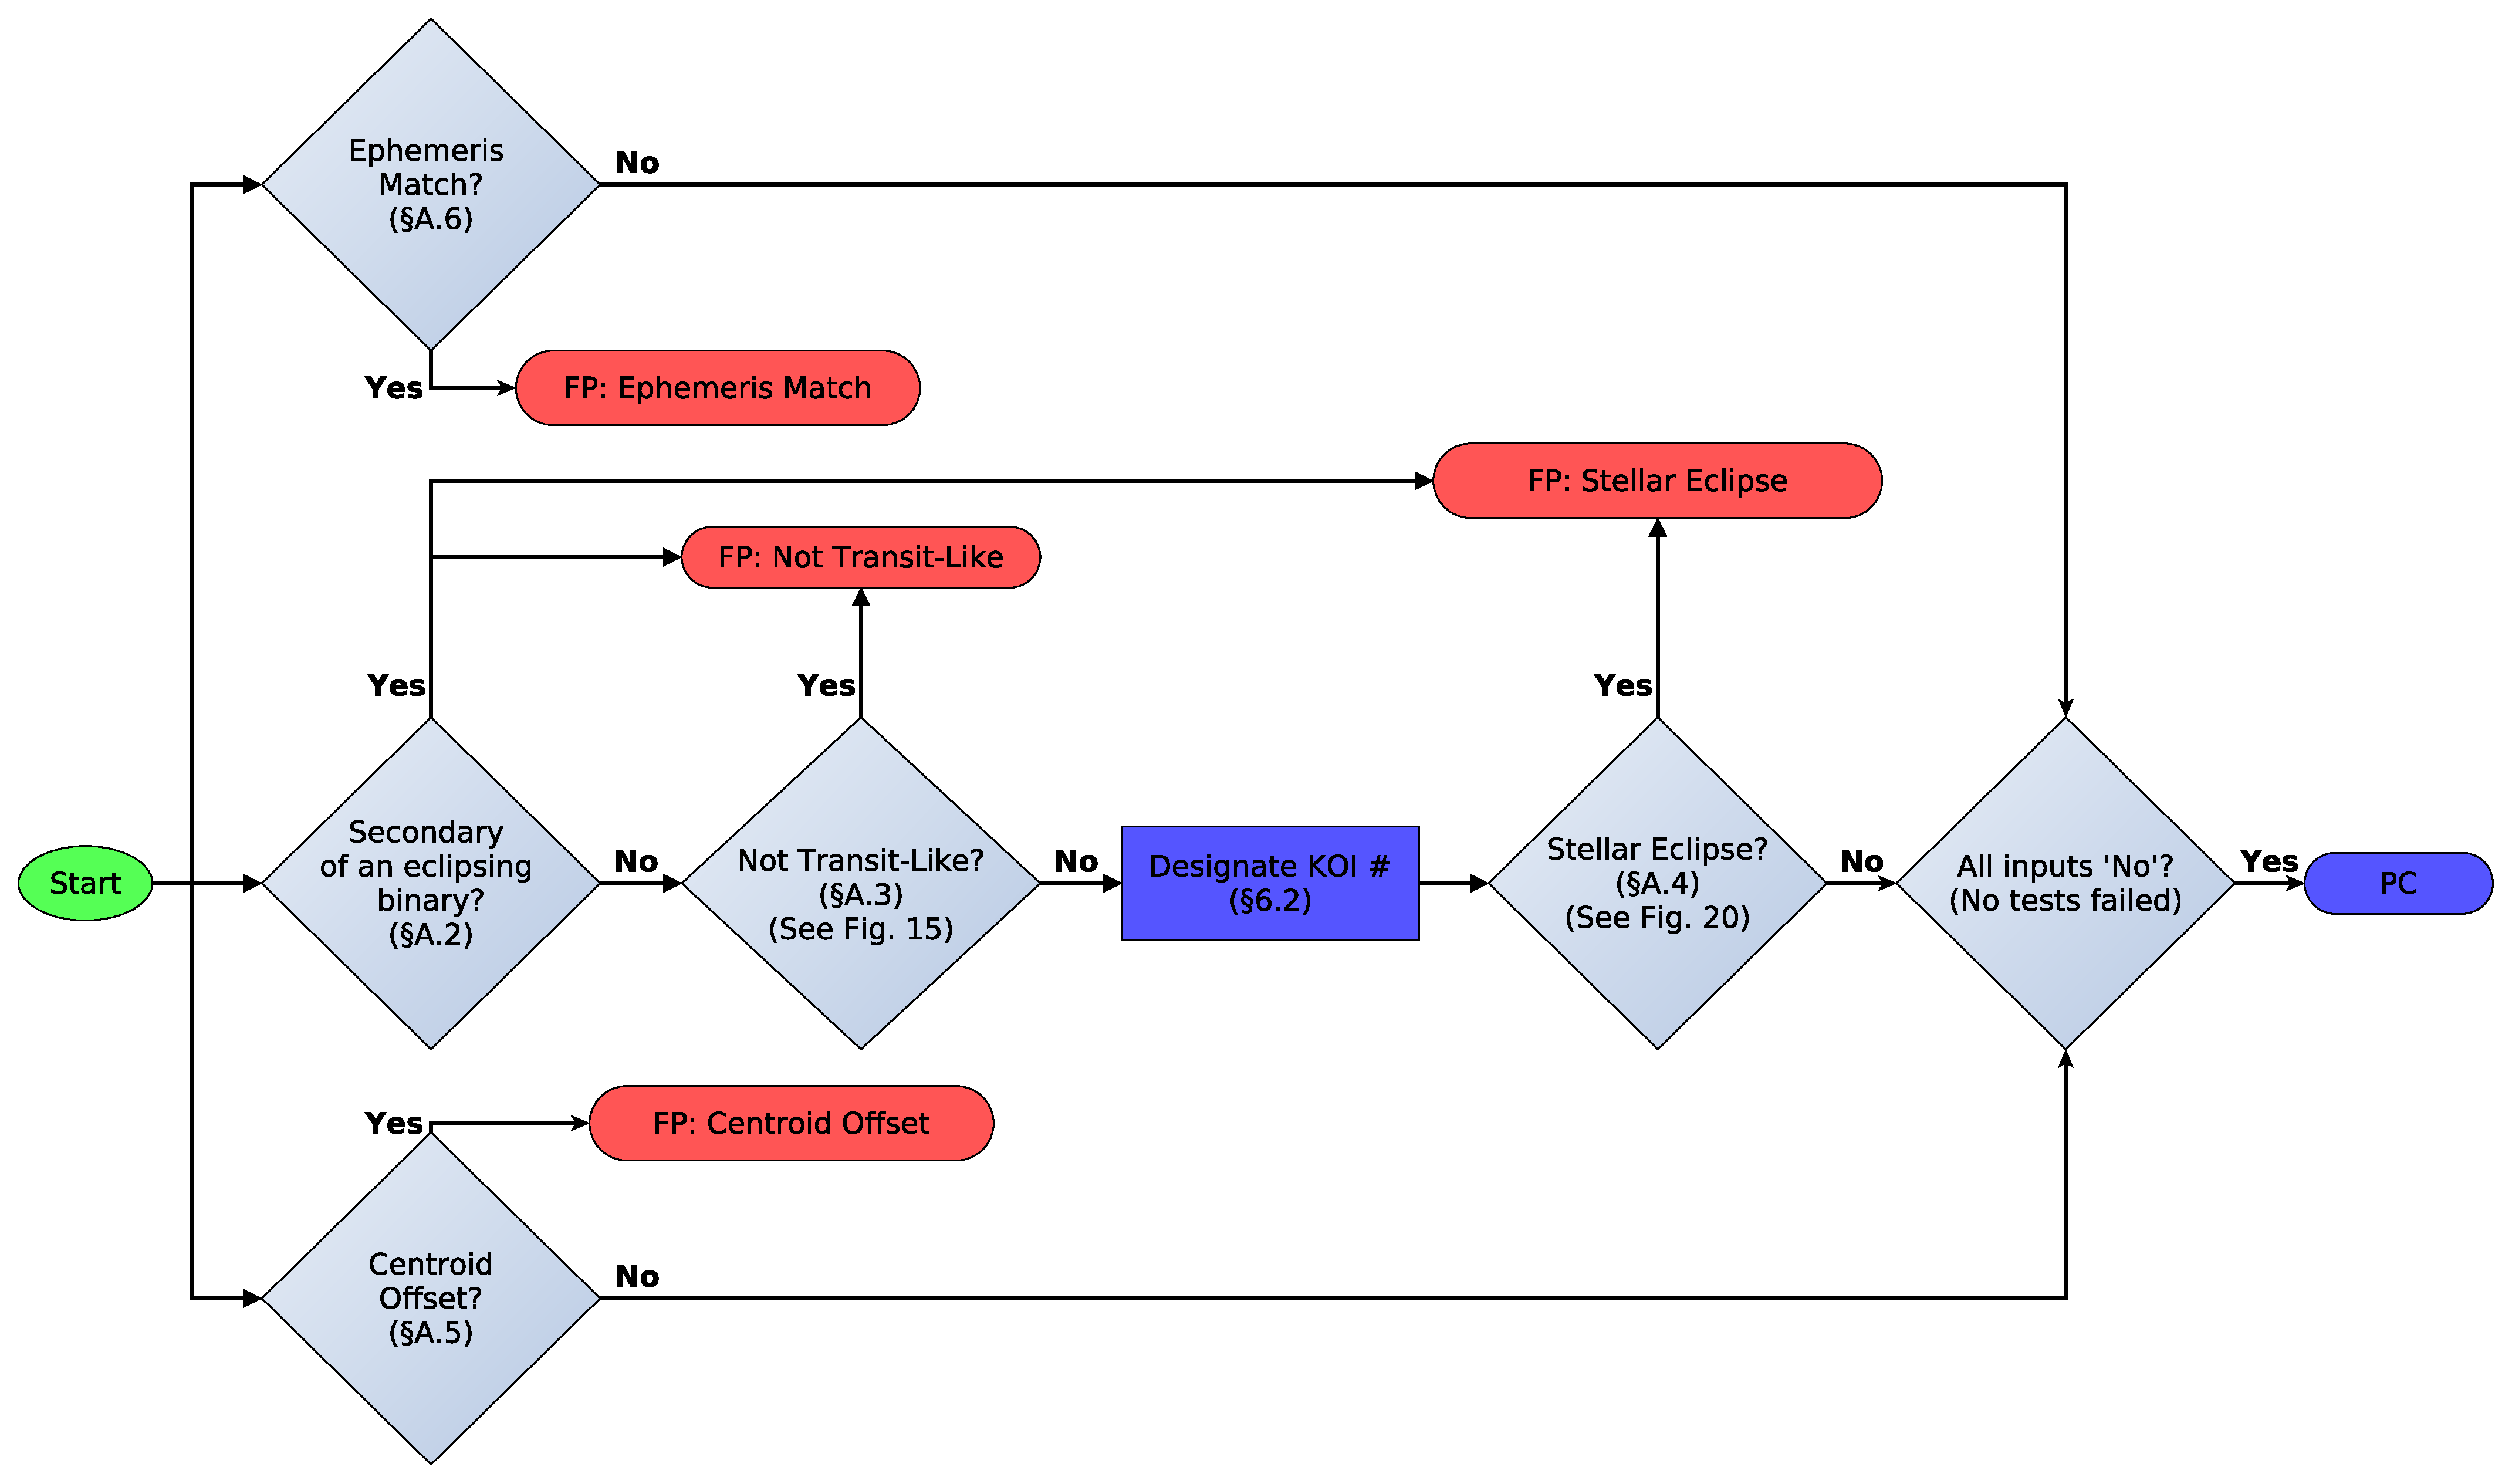
\includegraphics[width=\linewidth]{RoboVetter-Diagram-V4-Overview.pdf}
\caption{Overview flowchart of the robovetter. Diamonds represent ``yes'' or ``no'' decisions that are made with quantitative metrics. A TCE is dispositioned as a FP if it fails any test (a ``yes'' decision) and is placed in one or more of the FP categories. If a TCE passes all tests (a ``no'' decision for all tests) it is dispositioned as a PC. The section numbers on each component correspond to the sections in this paper where these tests are discussed. ***UPDATE SECTION HEADERS WHEN PAPER IS NEAR FINAL***. More in-depth flowcharts are provided for the not transit-like and significant secondary modules in Figures~\ref{robovetter-transitlike-fig} and \ref{robovetter-sigsec-fig}.}
\label{robovetter-overview-fig}
\end{figure*}


We note that for all of the robovetter tests that require a phased light curve and model fit, we utilize two different detrendings and model fits. In the \kepler{} pipeline, the Data Validation (DV) module produces a harmonic-removed, median-detrended, phased flux light curve, along with a transit model fit \citep{Wu2010}. However, the harmonic remover is known to suppress short-period ($\lesssim$ 3 days) signals such that short-period eclipsing binaries with visible secondaries can appear as transiting planets with no visible secondary \citep{Christiansen2013b}. It can also make variable stars with semi-coherent variability, such as starspots or pulsations, appear as transit-like signals. Thus, we create phased flux light curves via an alternate detrending method that utilizes the pre-search data conditioned (PDC) time-series light curves and the non-parametric penalized least squares detrending method of \citet{Garcia2010}, which includes only the out-of-transit points when computing the filter. These alternately detrended light curves are then phased and fit with a simple trapezoidal transit model. This alternate detrending technique is effective at accurately detrending short-period eclipsing binaries and variable stars, i.e., preserving their astrophysical signal. Every test that is applied to the DV phased light curves is also applied to the alternate detrending --- failing a test using either detrending results in the TCE being classified as a FP.

The robovetter first checks if the TCE corresponds to a secondary eclipse associated with an already examined system. If not, the robovetter then checks if the TCE is transit-like or not. If it is transit-like, the robovetter then looks for the presence of a secondary eclipse. In parallel, the robovetter also looks for evidence of a centroid offset and an ephemeris match to other TCEs and variable stars in the \kepler{} field. In the following subsections we describe in detail each of these tests in the order in which they are performed by the robovetter. Finally, we explain the creation of a ``disposition score'' that conveys the confidence in the Robovetter's disposition.


\subsection{The TCE is the Secondary of an Eclipsing Binary}

If a TCE under examination is not the first one in a system, the robovetter checks if there exists a previous TCE with a similar period that was designated as a FP due to a significant secondary (see~\S\ref{sigsecsec}). To compute whether two TCEs have the same period within a given statistical threshold, we employ the period matching criteria of \citet[][see equations 1-3]{Coughlin2014a}, $\sigma_{P}$, where higher values of $\sigma_{P}$ indicate more significant period matches. We re-state the equations here as:

\begin{equation}
\label{peq1}
\Delta P = \frac{P_{A}-P_{B}}{P_{A}}\\
\end{equation}

\begin{equation}
\label{peq2}
\Delta P^{\prime} = \textrm{abs}(\Delta P - \textrm{rint}(\Delta P))\\
\end{equation}

\begin{equation}
\label{peq3}
\sigma_{P} = \sqrt{2}\cdot\textrm{erfcinv}(\Delta P^{\prime})\\
\end{equation}

\noindent where $P_{A}$ is the period of the shorter-period TCE, $P_{B}$ is the period of the longer-period TCE, $rint()$ rounds a number to the nearest integer, $abs()$ yields the absolute value, and erfcinv() is the inverse complementary error function. We consider any value of $\sigma_{P}$ $>$ 3.5 to indicate significantly similar periods.

If the current TCE is (1) in a system that has a previous TCE dispositioned as a FP due to a significant secondary, (2) matches the previous TCE's period with $\sigma_{P}$ $>$ 3.5, and (3) is separated in phase from the previous TCE by at least 2.5 times the transit duration, then the current TCE is considered to be a secondary eclipse. In this case, it is designated as a FP and is classified into both the not transit-like and significant secondary FP categories --- a unique combination that can be used to identify secondary eclipses while still ensuring they are not assigned \kepler{} Object of Interest numbers (see \S\ref{koisec}). Note that since the \kepler{} pipeline identifies TCEs in order of their SNR, from high to low, sometimes a TCE identified as a secondary can have a deeper depth than the primary, depending on their relative durations and shapes.

There are two cases where we modify the three criteria above. First, it is possible that the periods of two TCEs will meet the period matching criteria, but be different enough to have their relative phases shift significantly over the $\sim$4 year mission duration. Thus, the potential secondary TCE is actually required to be separated in phase by at least 2.5 times the previous TCE's transit duration over the entire mission time frame in order to be labeled as a secondary. Second, the \kepler{} pipeline will occasionally detect the secondary eclipse of an EB at a half, third, or some smaller integer fraction of the orbital period of the system, such that the epoch of the detected secondary coincides with that of the primary. Thus, for the non-1:1 period ratio cases, we do not impose the phase separation requirement. (Note that equations~\ref{peq1}-\ref{peq3} allow for integer period ratios.)



\subsection{Not Transit-Like}
\label{nottransitlikesec}

A very large fraction of false positive TCEs have light curves that do not resemble a detached transiting or eclipsing object. These include quasi-sinusoidal light curves from pulsating stars, starspots, and contact binaries, as well as more sporadic light curves due to instrumental artifacts. The first step in the catalog process is to determine whether each TCE is not transit-like, or if it should be given \kepler{} Object of Interest (KOI) numbers, which are used to keep track of transit-like systems over multiple \kepler{} pipeline runs. We thus employ a series of algorithmic tests to reliably identify these not transit-like FP TCEs, as shown by the flowchart in Figure~\ref{robovetter-transitlike-fig}.


\begin{figure*}[ht]
\centering
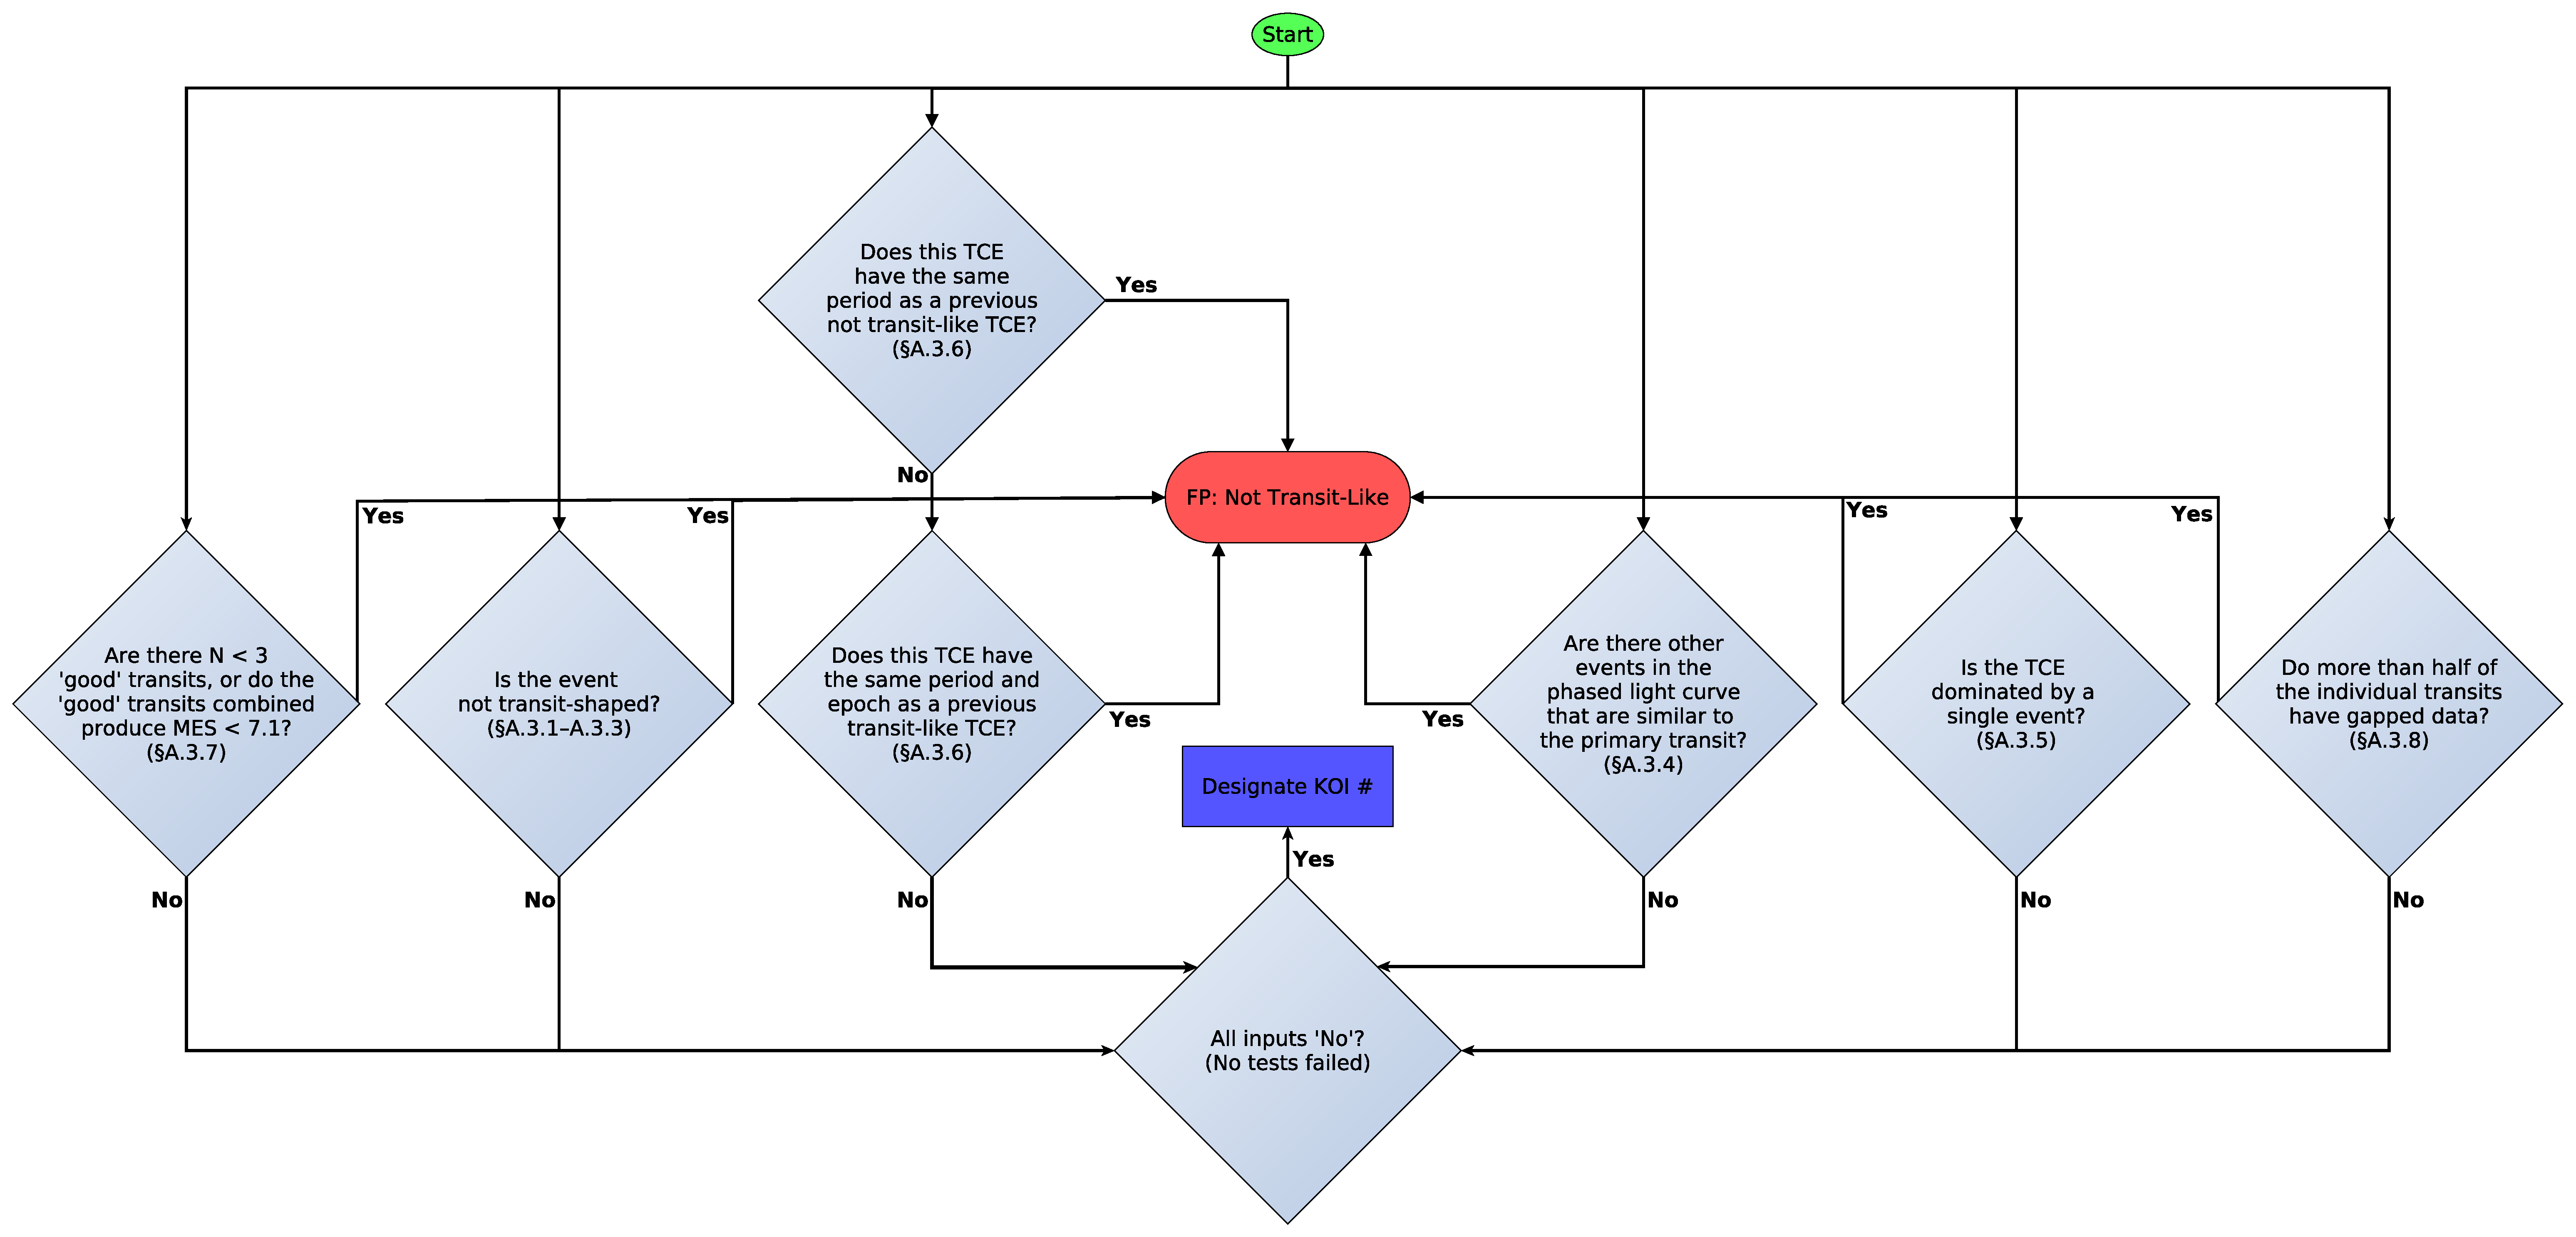
\includegraphics[width=\linewidth]{RoboVetter-Diagram-V4-TransitLike.pdf}
\caption{Not transit-like flowchart of the robovetter. Diamonds represent ``yes'' or ``no'' decisions that are made with quantitative metrics. If a TCE fails any test (via a ``yes'' response to any decision) then it is dispositioned as a not transit-like FP. If a TCE passes all tests (via a ``no'' response to all decisions), then it is given a KOI number and passed to the significant secondary module (see \S\ref{sigsecsec} and Figure~\ref{robovetter-sigsec-fig}). The section numbers on each decision diamond correspond to the sections in this paper where these tests are discussed.}
\label{robovetter-transitlike-fig}
\end{figure*}


\subsubsection{Not Transit-Shaped}

One of the most common false positives in the data set are quasi-sinusoidal shaped light curves, compared to those that are more detached due to a transit or eclipse. Also, individual events can often be due a systematic feature, such as a sudden discontinuity in the light curve. As such, the robovetter employs tests that detect quasi-sinusoidal light curves and systematics.


\paragraph{The LPP Metric}
\label{lppsec}

Many short-period false positives are due to variable stars that exhibit a quasi-sinusoidal phased light curve. We implemented the LPP transit-like metric described by \citet{Thompson2015b} to separate those TCEs that show a transit shape from those that do not. This technique bins the TCE's folded light curve and then applies a dimensionality reduction algorithm called Locality Preserving Projections (LPP) \citep{}.  It then measures the average Euclidean distance to the nearest known transit-like TCEs to yield a single number that represents the similarity of a TCE's shape to that of known transits. 

For the DR25 KOI catalog, we deviated slightly from the method described by \citet{Thompson2015b}.  This was done to solve the problem that the LPP metric was highly dependent on both period and MES. The empirical LPP metric threshold increases at periods less than a few days. This is caused by the fact these TCEs transit for a large fraction of the orbital period and thus have a different transit shape. Because transit injection does not include a large number of this type of event, the LPP values for good transits can be larger.  The trend with MES is routed in the fact that when the binned light curve has a lower signal to noise, it is less likely for two folded light curves to be similar to each other, creating more scatter in the final metric. 

To calculate the LPP metric we start with detrended \kepler{} light curves. (Note we calculated the metric for both detrendings discussed above.)  When training the LPP algorithm, we used the set of recovered transit injection TCEs and those planet candidates from the DR24 catalog \citep{Coughlin2016cat} that were found as TCEs in DR25.  Because we injected very few short period transits, including the short period DR24 candidates helped reduce the dependence of the LPP metric on period.  Also, we changed how the folded light curve was binned. To remove some of the MES dependence, TCEs with lower MES are given wider bins for those near the transit center; note, this does not change the number of bins. Because it yielded better performance, we used 97?? bins in total to represent the shape of the light curve.  Finally, we divided the raw LPP values by the 75$^{th}$ percentile of the N?? TCEs that are closest in period. (Did we also do this in MES?) In this way we further remove the period dependence on the LPP metric.  The resulting LPP metric values lie near a value of one where values greater than $\approx$ 2 do not appear transit-like.  

%Begin Jeff's words.
%Many short-period false positives are due to variable stars that exhibit a quasi-sinusoidal phased light curve. \citet{Matijevic2012} used a technique known as Local Linear Embedding (LLE), a dimensionality reduction algorithm, to classify the ``detachedness'' of \kepler{} eclipsing binary light curves on a scale of 0 to 1, where 0 represented fully detached systems with well-separated, narrow eclipses and 1 represented contact binaries with completely sinusoidal light curves. We use a similar technique, known as Local Preserving Projections \citep[][LPP]{He2004}, to distinguish transit-like signals from not transit-like signals \citep{Thompson2015b}. LPP returns a single number that represents the similarity of a TCE's shape to that of known transits. Unlike LLE, LPP can be applied to any TCE, not just those that lie within the parameter space of the training set. Thus, LPP is more suitable for separating transit-like TCEs from all other not transit-like TCEs, and can be run on artificially injected transits.


%We then fold and bin each light curve into 141 points, ensuring adequate coverage of both the in- and out-of-transit portions of the light curve. We exclude points near a phase of 0.5, as the presence of a secondary eclipse in a short-period binary may unduly influence the LPP value, and we seek to classify detached eclipsing binaries as transit-like. These 141 points act as the initial number of dimensions that describe each TCE. Using a subset of known transit-like TCEs, we create a map from the initial 141 dimensions down to 20 dimensions. We apply this map to all TCEs and measure the average Euclidean distance of each to the 15 nearest known transit-like TCEs. This average distance is the value of the LPP metric. When small, it means other transit-like TCEs are nearby in the 20 dimensional space and thus is likely to be shaped like a transit. We calculate this LPP transit metric for all TCEs using both the DV and the alternate detrending, as described in \S\ref{nottransitlikesec}.

%SUSAN - DESCRIBE HERE HOW YOU NORMALIZED THE LPP VALUES W.R.T. PERIOD, etc. 

% OLD TEXT DESCRIBING THE CHOICE OF THRESHOLD. Now we just adjust.
%
% In order to quantitatively determine a threshold between transit-like and not transit-like, we run the LPP classifier on both detrendings of the injected transits (see \S\ref{injectsec}), which we know a priori are all transit-shaped, barring any light curve distortion due to detrending. We then fit a Gaussian to the resulting distribution, computing its median and standard deviation. We then select a maximum LPP cutoff such that we expect less than one false negative in \ntces{} TCEs, via 

% \begin{equation}
% \sigma_{\rm LPP} = \sqrt{2}\cdot \textrm{erfcinv}(1/N_{\rm TCEs})
% \end{equation}

% \noindent where $N_{TCEs}$ = \ntces{}, yielding $\sigma_{\rm LPP}$ = 4.06. Any TCE with a LPP value greater than the median plus 4.06 times the standard deviation, using either detrending, is considered not transit-like.



\paragraph{Sine Wave Event Evaluation Test}
\label{sweetntlsec}

On occasion, a quasi-sinusoidal variable star will appear as transit-like in both the DV and ALT detrendings. In these cases, the only way to detect that the TCE is a FP is by examining the PDC data and looking for a strong quasi-sinusoidal signal at the TCE's period. We thus invented the Sine Wave Event Evaluation Test (SWEET) to identify these types of FPs.

SWEET takes the PDC data and normalizes each quarter by dividing by the median flux value of that quarter, then subtract 1.0. Outliers are then robustly removed by utilizing the median absolute deviation. Three different sine curves are then fit to the resulting data, with their periods fixed to half, exactly, and twice the TCE period, with their phase, amplitude, and offset allowed to vary. Of the three fits, the one with the highest SNR, defined as the amplitude divided by its error, is chosen as the strongest fit. If a TCE has a SWEET SNR greater than 50, an amplitude greater than the TCE transit depth in both the DV and ALT detrendings, and has a period less than 5.0 days, it fails a not transit-like.

% Can provide exact outlier rejection formula if desired, but seemed unnecessary



\paragraph{Per-TCE CHASES}

NEED TEXT FROM CHRIS









\subsubsection{The Model-Shift Uniqueness Test}
\label{notuniquetcesec}

If a TCE under investigation is truly a PC, there should not be any other transit-like events in the light curve with a depth, duration, and period similar to the primary signal, in either the positive or negative flux directions, i.e., the transit event should be unique in the phased light curve. Many false positives are due to quasi-sinusoidal signals (see \S\ref{tcesec}) and thus are not unique in the phased light curve. In order to identify these cases, TCERT developed a ``model-shift uniqueness test'' and used it extensively for identifying false positives in the Q1--Q12 \citep{Rowe2015a}, Q1--Q16 \citep{Mullally2015cat}, and DR24 \citep{Coughlin2016} planet candidate catalogs.

See \S3.2.2 of \citet{Rowe2015a} and page 20 of \citet{Coughlin2014b} for figures and a detailed explanation of the ``model-shift uniqueness test'', but in brief, after removing outliers, the best-fit model of the primary transit is used as a template to measure the best-fit depth of the transit model at all other phases. The deepest event aside from the primary (pri) transit event is labeled as the secondary (sec) event, the next-deepest event is labeled as the tertiary (ter) event, and the most positive (pos) flux event (i.e., shows a flux brightening) is labeled as the positive event. The significances of these events ($\sigma_{\rm Pri}$, $\sigma_{\rm Sec}$, $\sigma_{\rm Ter}$, and $\sigma_{\rm Pos}$) are computed assuming white noise as determined by the standard deviation of the light curve residuals. Also, the ratio of the red noise (at the timescale of the transit duration) to the white noise ($F_{\rm Red}$) is computed by examining the standard deviation of the best-fit depths at phases outside of the primary and secondary events.  

When examining all events among all TCEs, assuming Gaussian noise, the minimum threshold for an event to be considered statistically significant is given by

\begin{equation}
    FA_{1} = \sqrt{2}\cdot \textrm{erfcinv}\left(\frac{T_{\rm dur}}{P \cdot N_{\rm TCEs}}\right)
\end{equation}

\noindent where $T_{\rm dur}$ is the transit duration, and $P$ is the period. (The quantity $P$/$T_{\rm dur}$ represents the number of independent statistical tests for a single target.) When comparing two events from the same TCE, the minimum difference in their significances in order to be considered distinctly different is given by

\begin{equation}
    FA_{2} = \sqrt{2}\cdot \textrm{erfcinv}\left(\frac{T_{\rm dur}}{P}\right)
\end{equation}

\noindent We thus compute the following quantities to use as decision metrics

\begin{equation}
    MS_{1} = FA_{1} - \sigma_{\rm Pri}/F_{\rm Red}
\end{equation}

\begin{equation}
    MS_{2} = FA_{2} - (\sigma_{\rm Pri} - \sigma_{\rm Ter})
\end{equation}

\begin{equation}
    MS_{3} = FA_{2} - (\sigma_{\rm Pri} - \sigma_{\rm Pos})
\end{equation}


In the robovetter, we disposition a TCE as a not transit-like FP if either $MS_{1}$~$>$~1.0, $MS_{1}$~$>$~2.0, or $MS_{1}$~$>$~4.0 in the DV detrending, or if either $MS_{1}$~$>$~-3.0, $MS_{1}$~$>$~1.0, or $MS_{1}$~$>$~1.0 in the alternate detrending. These criteria ensure that the primary event is statistically significant when compared to the systematic noise level of the light curve, the tertiary event, and the positive event, respectively. We also fail as not transit-like if $\sigma_{\rm Pri}$~==~0.0 in both the DV and alternate detrendings, i.e., their default values, which indicates a lack of fit in both detrendings, and thus something fundamentally flawed with the TCE.


\subsubsection{Dominated by Single Event}

The depths of individual transits of planet candidates should be equal to each other, and thus assuming constant noise levels, the SNR of individual transits should be nearly equivalent as well. In contrast, most of the long-period FPs that result from three or more equidistant systematic events are dominated in SNR by one of those events. The \kepler{} pipeline measures detection significance via the Multiple Event Statistic (MES), which is calculated by combining the Single Event Statistic (SES) of all the individual events that comprise the TCE --- both the MES and SES are measures of SNR. Assuming all individual events have equal SES values,

\begin{equation}
{\rm MES} = \sqrt{N_{\rm Trans}} \cdot {\rm SES}
\end{equation}

\noindent where $N_{\rm Trans}$ is the number of transit events that comprise the TCE. Thus, SES/MES = 0.577 for a TCE with three transits, and less for a greater number of transits. If the largest SES value of a TCE's transit events, ${\rm SES}_{\rm Max}$, divided by the MES is much larger than 0.577, this indicates that one of the individual events dominates when calculating the SNR.

In the robovetter, for TCEs with periods greater than 90 days, if ${{\rm SES}_{\rm Max} / {\rm MES} > 0.8}$ it is dispositioned as a not transit-like false positive. The period cutoff of 90 days is applied because short-period TCEs can have a large number of individual transit events, which dramatically increases the chance of one event coinciding with a large systematic feature, thus producing a large ${{\rm SES}_{\rm Max} / {\rm MES}}$ value despite being a valid planetary signal.

% The value of 0.8 was empirically chosen based on the results of transit injection (\S\ref{injectsec}) to reject a minimal number of valid planetary candidates, accounting for natural deviations of SES values due to light curve systematics and changes in local noise levels. 


\subsubsection{Previous TCE With Same Period}

Most quasi-sinusoidal false positives produce multiple TCEs at the same period, or at integer ratios of each other. If a TCE in a system has been declared as not transit-like due to another test, it is logical that all subsequent TCEs in that system at the same period, or ratios thereof, should also be dispositioned not transit-like. Thus, we match the period of a given TCE to all previous not transit-like FPs via equations~\ref{peq1}-\ref{peq3}. If the current TCE has a period match with $\sigma_{P}$ $>$ 3.25 to a prior not transit-like FP, it is also dispositioned as a not transit-like FP.

Similarly, some TCEs are produced that correspond to the edge of a previously identified transit-like TCE in the system. This often results when the previous TCE corresponding to a transit or eclipse is not completely removed prior to searching the light curve for another TCE. Thus, we match the period of a given TCE to all previous transit-like TCEs via equations~\ref{peq1}-\ref{peq3}.  If the current TCE has a period match with $\sigma_{P}$ $>$ 3.25 to a prior transit-like FP, and the two epochs are separated in phase by less than 2.5 transit durations, the current TCE is dispositioned as a not transit-like FP. For clarity, we note that it is sometimes possible that the periods of two TCEs will meet the period matching criteria, but be different enough to have their epochs shift significantly in phase over the $\sim$4 year mission duration. Thus, if they are separated in phase by less than 2.5 transit durations at any point in the mission time frame, the current TCE is dispositioned as a not transit-like FP.



\subsubsection{Individual Transit Metrics}

A new approach implemented in DR25 is to identify individual transit events for each TCE that are not actually due to a transit. After rejecting these `bad' transit events, we check if either

\begin{itemize}
\item There are less than 3 `good' events left
\item The re-computed MES using only `good' events is $<$ 7.1
\end{itemize}

\noindent If either of these conditions are met, then the TCE is failed as not transit-like This is in line with the \kepler{} mission requirement of at least three valid transit events with a MES~$\ge$~7.1 in order to generate a TCE. In the following subsections we list the various tests we apply to each individual transit event.


\paragraph{Rubble -- Missing Data}

A number of TCEs from the \kepler{} pipeline are based on transit events that are missing a significant amount of data either in-transit or just before and/or after. These tend to be false positives that are triggering on edges of gaps, or cases were a large amount of data has been removed and a TCE is being created from the residuals of previous TCEs in the system. We thus devised the ``Rubble'' metric to clean-up these remains from the TCE list. The Rubble value for each individual transit is computed by dividing the number of \Kepler\ cadences that are actually available by the number of cadences expected given \Kepler's regular 29.42\,min cadence.  We calculated Rubble across two transit durations centered on the epoch for each transit given the TCE's original linear ephemeris. 


\paragraph{Marshall -- Transit Shape}
\label{marshsec}
\citet{Coughlin2016} used the Marshall method \citep{Mullally16} to identify and reject false alarm TCEs caused by short period transients in the data. Marshall fits the proposed transit with models of a transit and various transients and used a Bayesian Information Criterion to decide which model was the best explanation for the data. Simulations in \citet{Mullally16} showed that Marshall was 95\% complete for TCEs with periods $>150$\,days and correctly rejected 66\% of simulated artifact events. The limit on Marshall's effectiveness at eliminating false alarms was it used a parabola to describe the out-of-transit flux, which failed to capture much of the real observed stellar variability. To ensure high completeness, Marshall was tuned to prevent a variable continuum causing true transits to be rejected, at the cost of a lower than ideal effectiveness.

For this catalog, we use a Gaussian Process approach \citep[GP][]{Rasmussen10} to provide an improved continuum model to improve our effectiveness while maintaining our high completeness. Briefly, our approach aims to model the covariance in the lightcurve to better fit the trends in our data.
A similar approach was used by \citet{ForemanMackey16} to model single transits due to very long period planets ($P > 1000$\,days).

Our procedure is as follows. For each individual proposed transit event, we select a snippet of PDC data 30 times the reported transit duration centered on the event. Where the event happens near the start (or end) of a quarter, we take a snippet of similar length anchored at the start (or end) of the quarter. We use the George package \citep{Ambikasaran14} to fit the covariance of the out-of-transit flux with an exponential squared function, $ {\mathrm{Cov(\delta t})} = A \exp{ (\delta t/\ell)^2}$, where $A$ and $\ell$ are tunable parameters. 

We next fit four models to the entire snippet.

\begin{equation}
\left.\begin{aligned}
G(t | A, \ell) + y_0 \\
G(t | A, \ell) + y_0 + S(t)\\
G(t | A, \ell) + y_0 + S(t)(1 - \exp{\beta t})\\
G(t | A, \ell) + y_0 + S(t - \tau/2) - S(t + \tau/2) 
\end{aligned}\right.
\end{equation}

\noindent
where $G$ is the Gaussian Process model with the tunable parameters held fixed to those found earlier, and $y_0$ is a constant offset. $S(t)$ is given by

\begin{equation}
S(t) = \frac{d}{1 - e^{-\gamma (t-t_0)} }
\end{equation}

\noindent
where $d$ and $t_0$ are tunable parameters, while $\gamma$ is held constant. This function, known as a sigmoid (or logistic) function, has a value of 1 for $t<t_0$, 0 for $t>t_0$, and transitions quickly, but smoothly, between the two states. By using a sigmoid and avoiding the discontinuities in present in the models used by the original Marshall algorithm we can use the L-BFGS-B algorithm \citep{Byrd95} available in the Scipy package \footnote{\url{www.scipy.org}} instead of the less robust Neldar-Mead.

The second function models a discrete jump in the data. We fit this model seeded with a negative-going dip at the predicted time of ingress, and also with a positive-going spike at the predicted egress, as we see both features in \Kepler\ data. The third model fits a Sudden Pixel Sensitivity Drop (SPSD) event, probably caused by a cosmic ray hit on the detection. The last model approximates a box transit. By varying the parameter $\gamma$ we could in principle model transit ingress and egress, but find that extra degree of freedom is not necessary to explain the low signal-to-noise events of most concern.

For each transit the Marshall method returns the BIC score, the preferred model and the difference between the preferred model and the sigmoid box fit.  A transit is considered sufficiently bad when the Marshall score exceeds a particular threshold, as with the original Marshall algorithm.  However, in a few cases the Gaussian processes fails, yield extremely large, unbelievable BIC values. In these cases the transit is set to always pass.  Also, for low MES transits, the expected SES of a transit is sufficiently low that Marshall will be unable to distinguish between the ``no transit" model and a low signal-to-noise transit.  Because of this the Robovetter uses the following logic when deciding whether a specific transit is not valid:



%Jeff's words.
%A number of long-period false positives are a result of three or more systematic events that happen to be equidistant in time and produce a TCE. There are two prominent types of systematic events in \kepler{} data: sudden pixel sensitivity dropouots (SPSDs) and step-wise discontinuities. SPSDs are due to cosmic ray impacts that temporarily reduce the detection sensitivity of the impacted pixels, resulting in a sudden drop in flux followed by an asymptotic rise back to the baseline flux level over a timescale of a few hours \citep{VanCleve2009}. Step-wise discontinuities are sudden jumps in the baseline flux level, in either the positive or negative flux direction, and are typically due to imperfect detrending, but may have other causes. If a TCE is due to several of these events that are of similar SNR, they will not be flagged as false positives without examining the shape of their individual events.

%ARE THERE MORE MODELS THAN JUST STEPWISE AND SPSD? WERE ANY ADDED IN DR25??  WHATS OFFSET ONLY - WE NEED TO DESCRIBE

%In order to detect TCEs due to SPSDs and step-wise discontinuities, we developed the ``Marshall'' metric \citep{Mullally2015b}. Marshall fits a transit, SPSD, and step-wise discontinuity model to each individual event of a long-period TCE. The Bayesian Information Criterion \citep[BIC;][]{Schwarz1978} is then used to select which model best fits each individual transit event given each model's number of degrees of freedom. 

If all of the following criteria are met

\begin{itemize}
\item The BIC of the best-fitting non-transit model is 10 lower than the BIC of the transit-model
\item The BIC of the best-fitting non-transit model is less than 1.0E6
\item Either MES/NREALTRANS $>$ 4.0 or the lowest BIC model is OffsetOnly.
\end{itemize}

\noindent then that event is determined to be due to a systematic rather than a transit, and labeled as a ``bad'' event. 

{\bf NEED TO MAKE SURE "NREALTRANS" IS DEFINED SOMEWHERE, AND OFFSET ONLY}


{\bf Add some kind of discussion of performance}
{\bf Add link to Source Forge code}


\paragraph{Chases -- SES artifacts}

NEED TEXT FROM CHRIS

Chris on KSO-447: I have only included events where an absolute value of the SES peak within 0.8 of the transit event SES is within 30\% of the analysis window. The analysis window is set to Porb/10.0.

``Chases'' looks at the TPS convolved light curve and measures the amount of ayssmetry in the SES time serires...=



\paragraph{Skye -- Image Artifacts}

As discussed in \ref{marshsec}, there are a number of TCEs caused due to rolling-band systematics. Since these systematics are due to imperfections in particular CCDs, they are seen on different targets on the same CCD at about the same time. Thus, if a number of individual transit events from TCEs on different targets, but the same skygroup, occur at the same time, they are very likely systematic in origin. We thus invented a metric called ``Skye'' that looks for excess numbers of individual events occurring at the same time in the same skygroup, such that we can identify these individual transit events as systematic in origin.

% CHECK IF THE TERM 'SKYGROUP' HAS BEEN DEFINED PREVIOUSLY. IF NOT, DEFINE IT HERE.

We start by selecting only TCEs with periods greater than 45 days ($\sim$half a quarter) for each skygroup. The reason for the period cut is that long-period TCEs are most likely to be affected by rolling-band systematics, and that including shorter period TCEs would dramatically increase the number of individual transits, making it difficult to identify transit time clusters. We create a histogram of all these TCEs' individual transit times in 1.0 day bins. We also compute the average number of transits per time bin, or the \emph{rate}, by dividing the overall number of transit times in the skygroup by the number of bins. Assuming the majority of transits are randomly distributed in time, and utilizing Poisson counting statistics, any peaks greater than:

\begin{equation}
threshold = rate + sigma*\sqrt{rate}
\end{equation}

\noindent are statistically significant and indicative of temporal clustering, given a chosen \emph{sigma} value. We choose a value of \emph{sigma} = 3.0, and robustly determine the rate for each skygroup by first computing the \emph{threshold} using all the bins, then iteratively rejecting all bins with a height greater than \emph{threshold} and re-computing \emph{threshold} until it converges and does not change with further iterations.

For each skygroup and its threshold, we identify the individual times of transit for TCEs belonging to the skygroup that fall in bins that are above the threshold. We assign Skye values of 1 to these individual events to indicate they are 'bad'. The Skye value for all other transit times are set to 0. An example is shown in Figure~\ref{skyefig}.

\begin{figure}[h]
\centering
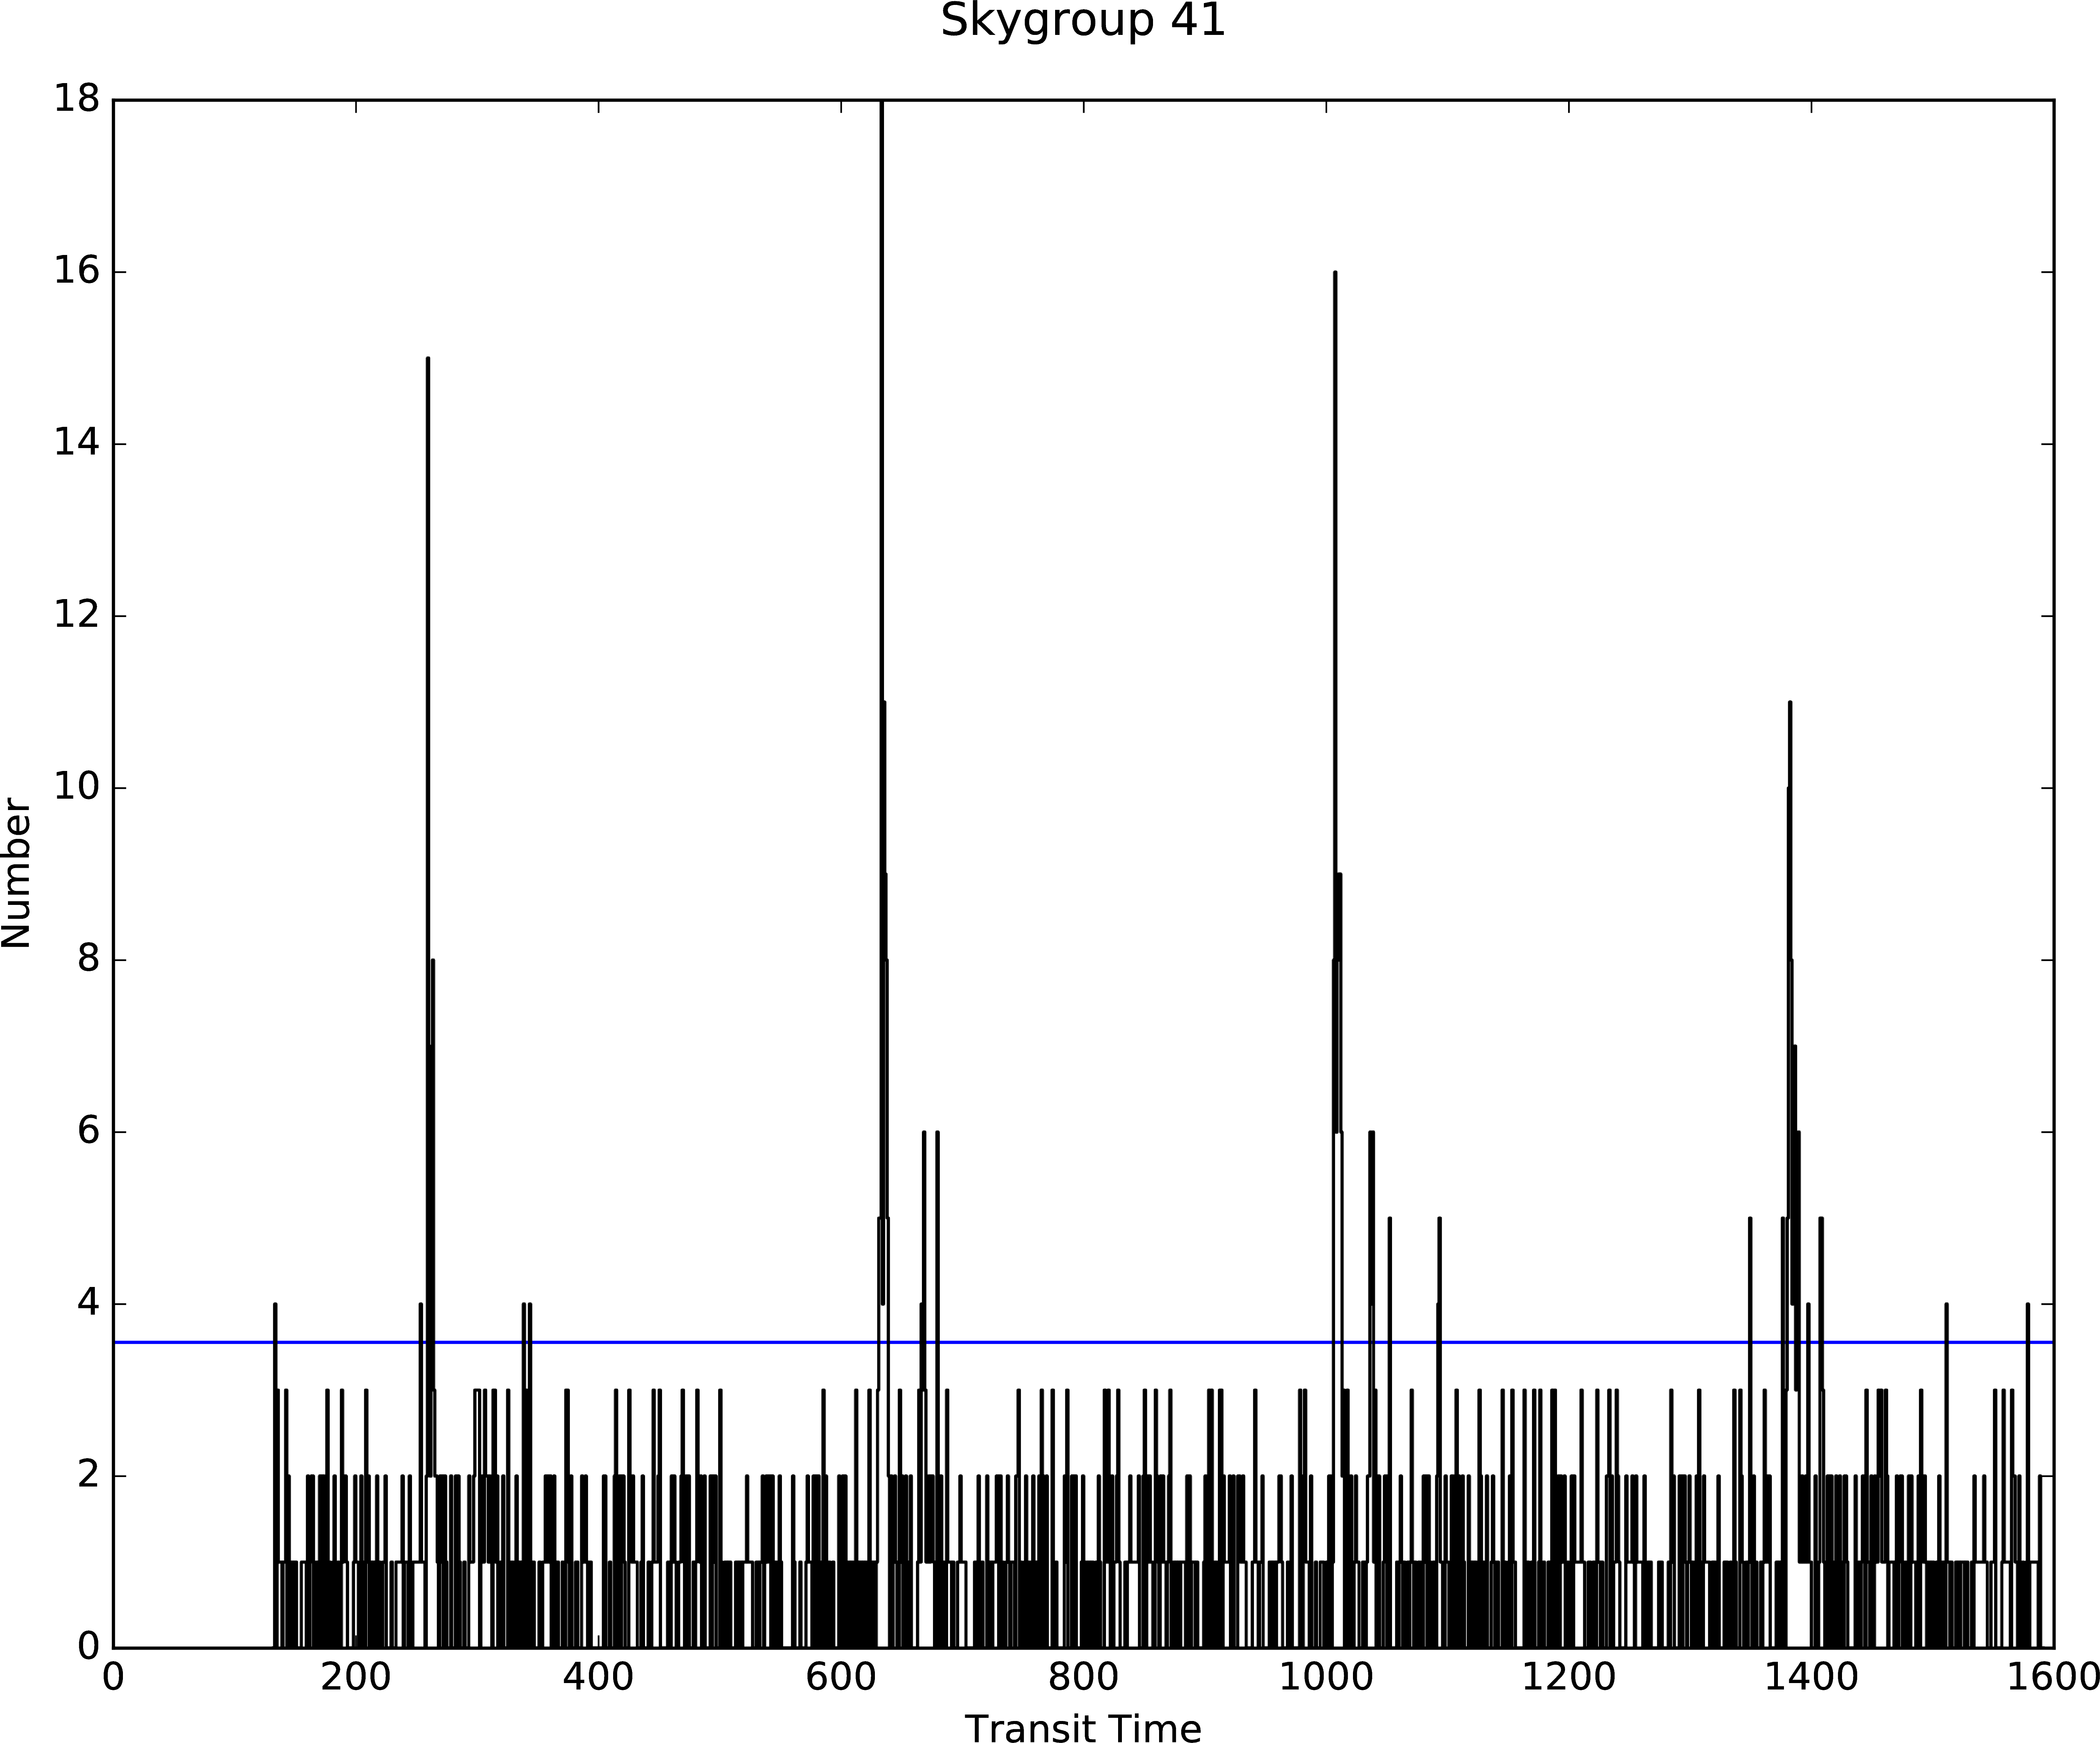
\includegraphics[width=\linewidth]{Skye-Paper-Plot.png}
\caption{Skye Example. Will need to update a some point.}
\label{skyefig}
\end{figure}

%Susan's words
%The Skye metric searches for those transit times that have an unusual number of transits at the same time on the same skygroup.   One well known image artifact is called rolling band. \textbf{When two frequencies beat together they create something that is described in the instrument handbook it creates changes in the black level that are both time and spatial dependent.} This effect should cause many transit like events to occur at approximately the same time for all stars on that channel when rolling band occurs. Because the telescope rolls every once each quarter, these rolling band artifact conspire to create TCEs around 370\,d in period.  The Skye metric examines the skyline plot, see Figure\label{f:skyline} for an example, for each skygroup and identifies those times with an excess of transits in a one day bin.  All transits that fall in this bin are marked as an invalid transit.

%Skye chooses the threshold for each skygroup with the following logic.  For each skygroup the average rate of transits per time bin is found by taking the number of transits associated with TCEs with Periods less than 40?? days. One day bins are created running from 200?? to 1600??, skipping any bin which no transits exist using the entire population of OBS TCEs, this removes time bins for which no data exists for the majority of targets.  The average rate of transits per bin (R) is given by the number of transits (N) divided by the number of bins (B) and the scatter in that average would likely be governed by Poisson statistics.  We define a threshold as $R + S \times \sqrt{R}$ where S is an arbitrary value that is held constant for all skygroups.  Since some transits are known to be clustered, these transits will not contribute evenly to all the bins and create a high value for R. To adjust for this we iteratively remove the transits in bins that are above the threshold and then recalculate R using the new values for both the remaining number of transits and the remaining number of bins. We stop iterating when there are no more peaks and the values converge.

\paragraph{Zuma -- Negative Significance}

A valid transit-like TCE should be comprised of individual events that correspond to flux decrements. If any event instead shows an increase of flux then that event is suspect. We thus designate any individual event with SES~$<$~0 as `bad'.


\paragraph{Tracker -- Ephemeris Slip}

After the TPS module of the \kepler{} pipline detects a TCE, it is sent to to DV to be fit with a full transit model. DV allows the period and epoch to vary when fitting in order to provide as accurate a fit as possible. Sometimes the TPS ephemeris and DV ephemeris can end up significantly different though. When this occurs it indicates that the underlying data is not transit-like and the TCE is likely due to quasi-sinusoidal systematics, which case the ephemeris to wander when fitting.

``Tracker'' keeps track of the time difference between the TPS and DV linear ephemerides in units of the TCE's duration. When Tracker $>$ 0.5 for any event we designate the event as 'bad'.


% The metric formally known as Rocky
\subsubsection{TCE Dominated by Gapped Events}

Due to the method of data gapping employed in TPS, sometimes the \kepler{} pipeline can create a TCE that has a majority of its individual events occur where there is no actual in-transit data. This tends to happen particularly in multi-TCE systems, as once the \kepler{} pipline detects a TCE in a given system, it removes the data corresponding to the in-transit cadences of that TCE, and re-searches the light curve. 

We thus developed a metric that measures the number of individual transit events that actually contain data. Specifically we compute the fraction of individual events with either SES~$\ne$~0 or Rubble~$>$~0.75, which indicate there is sufficient in-cadence data present. If the fraction of transits with data is~$\le$~0.5, then we fail the TCE as not transit-like.





\subsection{Stellar Eclipse}
\label{sigsecsec}

If a TCE is deemed transit-like by passing all of the tests presented in \S\ref{nottransitlikesec} on both detrendings, it is given a KOI number. However, many of these KOIs are FPs due to eclipsing binaries and contamination from nearby variable stars. We employ a series of robotic tests to detect systems that are due to stellar companions, as shown by the flowchart in Figure~\ref{robovetter-sigsec-fig}.

%In order to produce a uniform catalog, we do not designate any TCE a FP on the basis of its transit depth or inferred radius --- see \S7 item 6 of \citet{Mullally2015cat} for more detail. 

% us, being agnostic to stellar parameters, the only way to definitively detect an EB via a \kepler{} light curve is by detecting a significant secondary eclipse. 

MENTION THE WHOLE SECONDARY -> STELLAR CHANGE, OR NOT?




\begin{figure*}[ht]
\centering
\includegraphics[width=\linewidth]{RoboVetter-Diagram-V3-SigSec.pdf}
\caption{Flowchart describing the stellar system tests of the robovetter. Diamonds represent ``yes'' or ``no'' decisions that are made with quantitative metrics. The multiple arrows originating from ``Start'' represent decisions that are made in parallel. NEED TO UPDATE!!}
\label{robovetter-sigsec-fig}
\end{figure*}


\subsubsection{Secondary Eclipse}

One of the most common methods to detect a stellar system is the presence of a significant secondary in the light curve. With the exception of some hot Jupiter type planets, the visibility of a secondary eclipse in \kepler{} data is a telltale sign of a stellar eclipsing binary.


\paragraph{Subsequent TCE With Same Period}

Once the \kepler{} pipeline detects a TCE in a given system, it removes the data corresponding to this event and re-searches the light curve. It is thus able to detect the secondary eclipse of an EB as a subsequent TCE, which will have the same period as, but different epoch than, the primary TCE. Thus, utilizing equations~\ref{peq1}-\ref{peq3}, the robovetter dispositions a TCE as a stellar system FP if its period matches a subsequent TCE within the utilized tolerance ($\sigma_{P}$ $>$ 3.25) and they are separated in phase by at least 2.5 times the transit duration. For clarity, we note again that it is sometimes possible that the periods of two TCEs will meet the period matching criteria, but be different enough to have their epochs shift significantly in phase over the $\sim$4 year mission duration. Thus, this phase separation requirement is required to be upheld over the entire mission duration in order to disposition the TCE as a FP due to a significant secondary.

Occasionally the \kepler{} pipeline will detect the secondary eclipse of an EB at half, third, or some smaller integer fraction of the orbital period of the system. In these cases, the epoch of the TCE corresponding to the secondary will overlap with that of the primary. These cases are accounted for by not requiring a phase separation of at least 2.5 transit durations when a period ratio other than unity is detected. (Note that equations~\ref{peq1}-\ref{peq3} allow for integer period ratios.) While this approach will likely classify any multi-planet system in an exact 2:1 orbital resonance as a FP due to a significant secondary, in practice this is non-existent. Exact 2:1 orbital resonances, where ``exact'' means the period ratio is close enough to 2.0 over the $\sim$4 year mission duration to avoid any drift in relative epoch, appear to be extremely rare \citep{Fabrycky2014}. Also, they would produce strong transit timing variations, which would likely preclude their detection. The \kepler{} pipeline employs a strictly linear ephemeris when searching for TCEs, and thus while planets with mild transit timing variations (TTVs), e.g., deviations from a linear ephemeris less than the transit duration, are often detected, planets with strong TTVs, e.g., deviations from a linear ephemeris greater than the transit duration, are often not detected.



\paragraph{Secondary Detected in Light Curve}
\label{secdetectsec}

There are many cases when a secondary eclipse does not produce its own TCE, most often when its MES is below the \kepler{} pipeline detection threshold of 7.1. The model-shift uniqueness test, discussed in \S\ref{notuniquetcesec}, is well-suited to automatically detect secondary eclipses in the phased light curve, as it searches for the next two deepest events aside from the primary event. It is thus able to detect the best-candidate secondary eclipse in the light curve and assess its significance. We thus compute the following quantities to use as secondary deteection metrics

\begin{equation}
    MS_{4} = \sigma_{\rm Sec}/F_{\rm Red} - FA_{1}
\end{equation}

\begin{equation}
    MS_{5} = (\sigma_{\rm Sec} - \sigma_{\rm Ter}) - FA_{2}
\end{equation}

\begin{equation}
    MS_{6} = (\sigma_{\rm Sec} - \sigma_{\rm Pos}) - FA_{2}
\end{equation}

If $MS_{4}$~$>$1, $MS_{5}$~$>$0, and $MS_{6}$~$>$0, in either the DV or alternate detrendings, the robovetter dispositions the TCE as a stellar system FP. These criteria ensure that the secondary event is statistically significant when compared to the systematic noise level of the light curve, the tertiary event, and the positive event, respectively.

There are two exceptions when the above-mentioned conditions are met, but the robovetter does not designate the TCE a false positive. First, if the primary and secondary are statistically indistinguishable, and the secondary is located at phase 0.5, then it is possible that the TCE is a PC that has been detected at twice the true orbital period. Thus, the robovetter labels a TCE with a significant secondary as a PC when ${\sigma_{\rm Pri} - \sigma_{\rm Sec} < FA_{2}}$ and the phase of the secondary is within 1/4 of the primary transit's duration of phase 0.5. Second, hot Jupiter PCs can have detectable secondary eclipses due to planetary occultations via reflected light and thermal emission \citep{Coughlin2012}. Thus, a TCE with a detected significant secondary is labeled as a PC with the significant secondary flag (in order to facilitate the identification of hot Jupiter occultations) when the geometric albedo is less than 1.0, the planetary radius is less than 30~\re{}, the depth of the secondary is less than 10\% of the primary, and the impact parameter is less than 0.95. The additional criteria beyond the albedo criterion are needed to ensure that this test is only applied to potentially valid planets and not grazing eclipsing binaries. We calculate the geometric albedo by using the stellar mass, radius, and effective temperature from \citet{Huber2014a}, and the values of the period and radius ratio from the DV module of the \kepler{} pipeline.



\paragraph{Odd/Even Depth Difference}

If the primary and secondary eclipses of an EB are similar in depth, and the secondary is located near phase 0.5, the \kepler{} pipeline may detect them as a single TCE at half the true orbital period of the EB. In these cases, if the primary and secondary depths are dissimilar enough, it is possible to detect it as a FP by comparing the depths of the odd- and even-numbered transit events. Thus, we compute the following statistic, for both the DV and alternate detrending,

\begin{equation}
\sigma_{\rm OE} = \frac{d_{\rm odd} - d_{\rm even}}{\sqrt{\sigma_{odd}^{2} + \sigma_{even}^{2}}} 
\end{equation}

\noindent where $d_{\rm odd}$ is the median depth of the odd-numbered transits, $d_{\rm even}$ is the median depth of the even-numbered transits, $\sigma_{odd}$ is the standard deviation of the depths of the odd-numbered transits, and $\sigma_{even}$ is the standard deviation of the depths of the even-numbered transits. For the alternate detrending with a trapezoidal fit, we use all points that lie within $\pm$30 minutes of the central time of transit, as well as any other points within the in-transit flat portion of the trapezoidal fit. For the DV detrending, we use all points within $\pm$30 minutes of the central time of transit. (This threshold corresponds to the long-cadence integration time of the \kepler{} spacecraft. Including points farther away from the central time of transit degrades the accuracy and precision of the test.) If $\sigma_{\rm OE}$ $>$ 1.7 for either the DV or alternate detrending then the TCE is labeled as a FP due to a significant secondary. The value of 1.7 was empirically derived utilizing manual checks and transit injection.


\subsubsection{Out of Eclipse Variability}

Short-period eclipsing binaries will often show out-of-eclipse variability due to tidal forces that deform the star from a perfect spheroid. The variability manifests as quasi-sinusoidal variations at either the period, or half the period, of the binary.

We use the information from SWEET (see~\S\ref{sweetntlsec}) to detect these cases. If a transit-like TCE has a SWEET SNR greater than 50, an amplitude less than the TCE transit depth in either the DV and ALT detrendings, an amplitude greater than 5,000~ppm, and a period less than 10 days, we fail it as a stellar system.



\subsubsection{Shape Metric}

There are cases of EBs that do not show a secondary eclipse, either due to the secondary star being too low luminosity for the eclipse to be detectable, or the binary has significant eccentricity and a longitude of periastron such that geometrically no eclipse occurs. Also, most detached EBs will not exhibit detectable out-of-eclipse variability. In these cases, the only remaining way to detect that the signal is due to a stellar system is to utilize the shape and depth of the transit to infer that the signal could not possible be due to a planet.

In previous catalogs \citep{Rowe2015cat,Mullally2015cat,Coughlin2016} TCEs were not failed based on their inferred radii alone. This was on purpose as the catalogs attempted to be as agnostic to stellar parameters as possible, such that dispositions would remain applicable if and when better stellar parameters were obtained, e.g., by GAIA \citep{Cacciari2009,Mignard2005}. This resulted in some PC KOIs with large depths that were known to very likely be EBs, and in fact were later confirmed as such by follow-up observations \citep{Santerne2016}.

In this catalog, we attempt to strike a balance between identifying these binary systems, while still remaining agnostic to stellar parameters. We adapted a simple shape parameter, originally used in \citet{Batalha2013}, and express it as the sum of the modeled radius ratio and the impact parameter. This metric reliability identifies eclipsing binaries both due to being too deep (large $R_{p}$/$R_{\star}$) and due to grazing eclipses (large $b$). Specifically we fail a transit-like TCE as a stellar system if $R_{p}$/$R_{\star}$~+~$b$~$>$~1.04.



\subsection{Centroid Offset}

Given that \keplers{} pixels are 3.98\arcsec{} square \citep{Koch2010}, and the typical photometric aperture has a radius of 4--7 pixels \citep{Bryson2010b}, it is quite common for a given target star to be contaminated by light from another star. If that other star is variable, then that variability will be visible in the target aperture at a reduced amplitude. If the variability due to contamination results in a TCE, then it is a false positive, whether the contaminator is an eclipsing binary, planet, or other type of variable star \citep{Bryson2013}. For example, if a transit or an eclipse occurs on a bright star, a shallower event will be observed on a nearby, fainter star. Similarly, a star can be mistakenly identified as experiencing a shallow transit if a deep eclipse occurs on a fainter, nearby source.

% There are two ways we robotically detect centroid offsets, by examining the differnce 


The DV module of the \kepler{} pipeline produces ``difference images'' for each quarter, which are made by subtracting the average flux in each pixel during each transit from the flux in each pixel just before and after each transit \citep{Bryson2013}. If the resulting difference image shows significant flux change at a location (centroid) other than the target, then the TCE is likely a FP due to a centroid offset.


% In prior catalogs, TCERT members manually examined the difference images to look for evidence of a centroid offset, as fully described in \citet{Bryson2013} and \S3.2.3--3.2.6 of \citet{Rowe2015a}. In this catalog, the search for centroid offsets was fully robotized and confirmed to reproduce the results earlier catalogs using human vetting \citep{Mullally2015c}.

In our robotic procedure to detect FPs due to centroid offsets, we first check that the difference image for each quarter contains a discernible stellar image and is not dominated by background noise. This is done by searching for at least 3 pixels that are adjacent to each other and brighter than a given threshold, which is set by the noise properties of the image. We use an iterative sigma clipping approach to eliminate bright pixels when calculating the background noise, as the star often dominates the flux budget of a substantial number of pixels in the aperture.

For the difference images that are determined to contain a discernible stellar image, we first search for evidence of contamination from sources that are resolved from the target. Since resolved sources near the edge of the image may not be fully captured, Pixel Response Function (PRF --- \keplers{} point spread function convolved with the image motion and the intra-pixel CCD sensitivity) fitting approaches do not often work well to detect them. Instead, we check if the location of the brightest pixel in the difference image is more than 1.5 pixels from the location of the target star. If at least two-thirds of the quarterly difference images show evidence of an offset by this criterion, we disposition the TCE as a FP due to a centroid offset. % Note that FPs due to stars located many pixels from the target, i.e., far outside the target's image, are not detected by this approach, but rather through ephemeris matching (see \S\ref{ephemmatchsec}).

If no centroid offset is identified by the previous method, we then look for contamination from sources that are unresolved from the target. We measure the PRF-fit centroid of the difference images and search for statistically significant shifts with respect to the PRF centroid of both the out-of-transit images, as well as the catalog position of the source. Following \citet{Bryson2013}, a TCE is marked as a FP due to a centroid offset if there are at least three difference images with a discernible stellar image, and a 3$\sigma$ significant offset larger than 2$\arcsec$, or a 4$\sigma$ offset larger than 1$\arcsec$ is measured.

Finally, the last method we use to detect a centroid offset the ghost diagnostic, which was added to the DR25 \kepler{} pipeline \citep{Twicken2016}. It determines whether a transit signal is likely to be contaminated from a ghost image of a star located away from the target star in the focal plane. Ghost reflections occur when light from a bright star is reflected from the CCD reflects again from the field flattener plate and back onto the CCD as a diffuse, out-of-focus image of the pupil of
the telescope. A similar type of false positive results from direct PRF (Pixel Response Function) contamination, when flux from the broad wings of the PRF of a bright star near the target star on the CCD overlaps the target star's PRF.  If a ghost reflection (or the PRF of a nearby star) containing a transit-like signature (e.g. an eclipsing binary signal) overlaps the PRF of a target star, then the contaminating transit signal will be significantly stronger relative to the target's flux in the periphery of the target star's PRF than in its core.


To detect this type of false alarm, the ghost diagnostic essentially measures the strength of the TCE signal in two separate light curves --- one created using the average of the pixels inside the target's optimal aperture minus the average of the pixels in an annulus surrounding the target aperture (core aperture correlation statistic), and the other using the average of the pixels in the annulus surrounding the target aperture (halo aperture correlation statistic). If the ratio of the out- to in-aperture statistic is greater than 4.0, the TCE is marked as a FP due to a centorid offset. This ghost diagnostic is not available for vetting the Scrambled TCEs.  

%Joe's words
% It produces a detection statistic measuring correlation between a whitened timeseries and a whitened transit model, as well as a statistic measuring the signicance of the correlation, assuming the detection statistic is a chi-squared variable.

\subsection{Ephemeris Matching}
\label{ephemmatchsec}

Another method for detecting FPs due to contamination is to compare the ephemerides (periods and epochs) of TCEs to each other, as well as other known variable sources in the \kepler{} field. If two targets have the same ephemeris within a specified tolerance, then at least one of them is a FP due to contamination. \citet{Coughlin2014a} used Q1--Q12 data to compare the ephemerides of KOIs to each other and eclipsing binaries known from both \kepler{}- and ground-based observations. They identified over 600 FPs via ephemeris matching, of which over 100 were not known as FPs via other methods. They also identified four main mechanisms of contamination. The results of \citet{Coughlin2014a} were incorporated in \citet[][see \S3.3]{Rowe2015a}. \citet[][see \S5.3]{Mullally2015cat} slightly modified the ephemeris matching process of \citet{Coughlin2014a}, and applied it to all of the Q1--Q16 TCEs, as well as known KOIs and EBs, identifying nearly 1,000 TCEs as FPs. The same process was again used in the \citet{Coughlin2016} catalog.

We modify the matching criteria used in previous catalogs to obtain more accurate matches, due especially to the very large number of long-period TCEs encountered in DR25 compared to previous activities. We utilize the results of the transit injection run (REF INJECTION SEC) to measure the ability of the \kepler{} pipeline to recover period and epoch as a function of period. In Figure~\ref{injephemfig} we show, in the top two panels, the difference in the injected and recovered period and epoch, as a function of the injected period. The middle and bottom panels show the measured standard deviation of the difference as a function of panel, in linear and logarithmic space respectively. The red line is the result of a best-fit power law.

\begin{figure}[h]
\centering
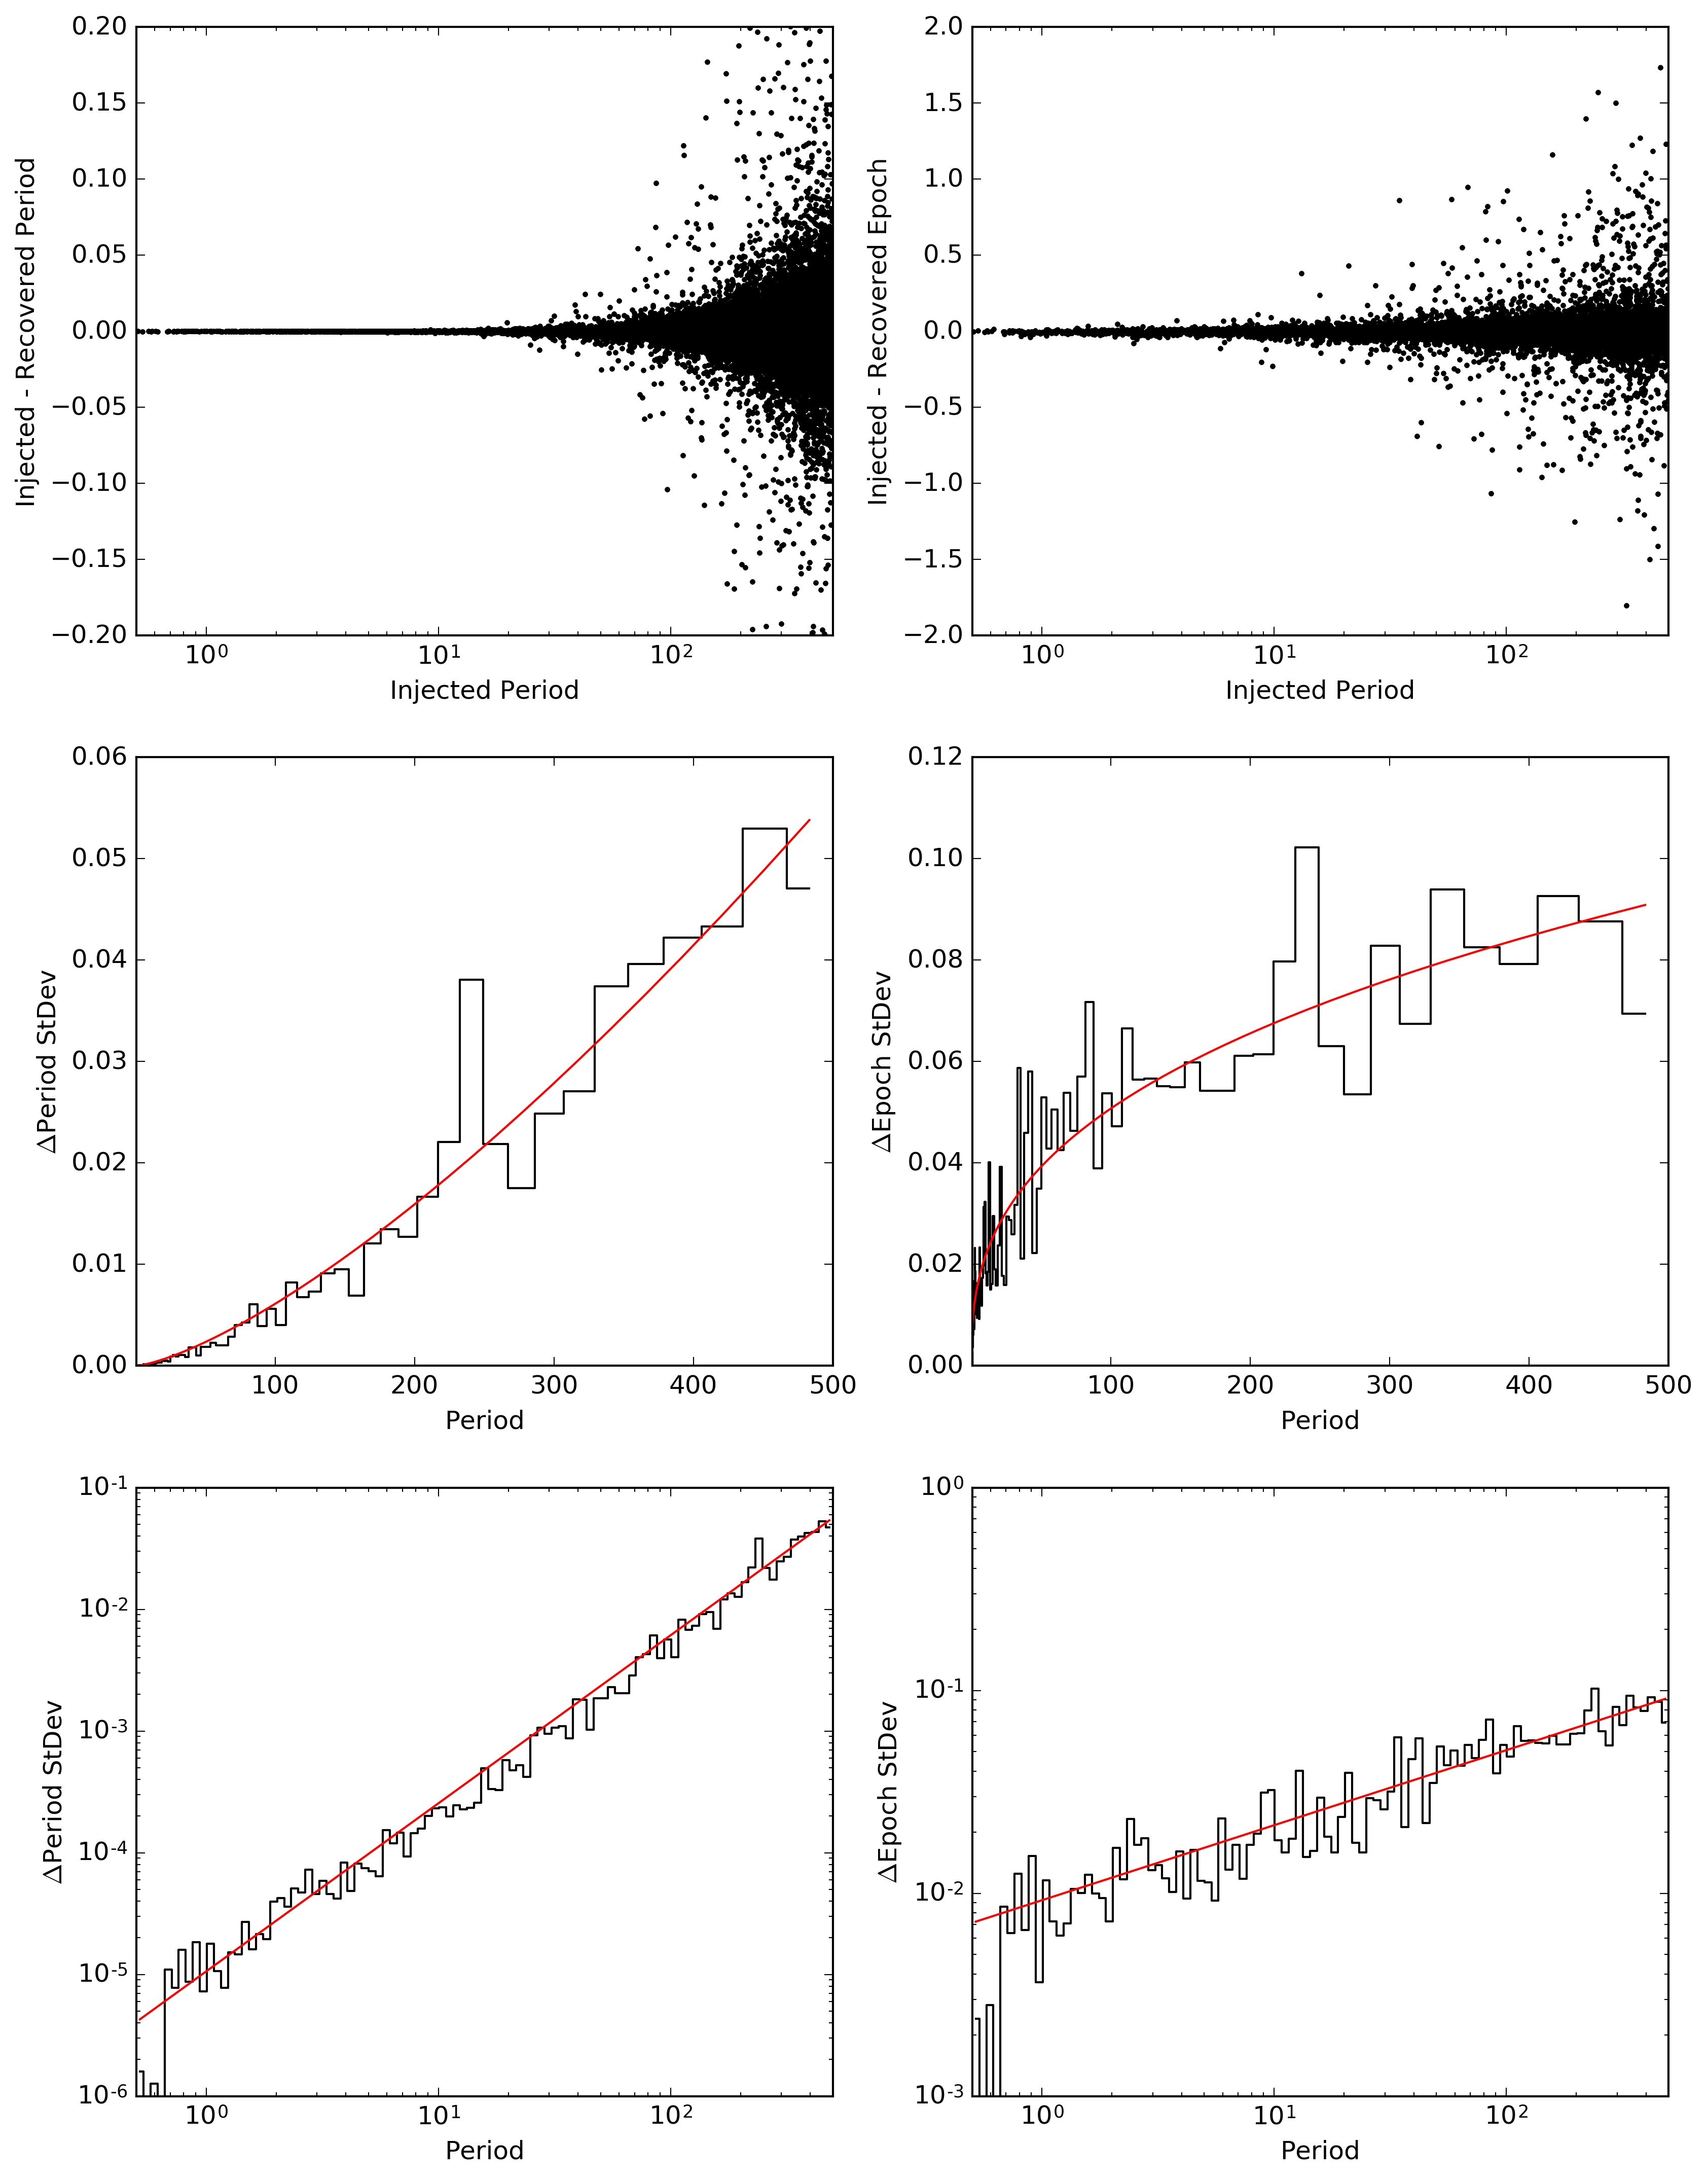
\includegraphics[width=\linewidth]{DR25-Injected-Vs-Recovered-Periods-And-Epochs.png}
\caption{A plot of injected vs. recovered periods and epochs of injected on-target planets. MAYBE UPDATE TO JUST 2x2 WITH ALL LOG-SCALE - I.E. KEEP BOTTOM PLOTS, TAKE OUT MIDDLE, AND MAKE TOP LOGSCALE.}
\label{injephemfig}
\end{figure}


When comparing two objects, A and B, where A is defined to have the shorter period, the new matching metrics we use, $S_{P}$ and $S_{T}$ for period and epoch respectively, are:

\begin{equation}
    S_{P} = \frac{\left|P_{r} \cdot P_{A} - P_{B}\right|}{\sqrt{2}\cdot\sigma_{P}(P_{A})}
\end{equation}

\begin{equation}
    S_{T} = \frac{\left| T_{A} - T_{B} - T_{r} \cdot P_{A}\right|}{\sqrt{2}\cdot\sigma_{T}(P_{A})}
\end{equation}

\noindent where $P_{A}$ and $P_{B}$ are the periods of objects A and B, $T_{A}$ and $T_{B}$ are similarly the epochs of objects A and B, $\sigma_{P}(P_{A})$ and $\sigma_{T}(P_{A})$ are the errors in period and epoch, given period $P_{A}$, derived from the best-fit power law to the standard deviation of the injected vs recovered periods and epochs, respectively, and the period ratio, $P_{r}$, and epoch ratio, $T_{r}$, are defined by:

\begin{equation}
P_{r} = \textrm{rint}\left(\frac{P_{A}}{P_{B}}\right)
\end{equation}

\begin{equation}
T_{r} = \textrm{rint}\left(\frac{T_{A} - T_{B}}{P_{A}}\right)
\end{equation}


\noindent where $rint()$ rounds a number to the nearest integer. Thus, a perfect match has $S_{P}$~=~0 and  $S_{T}$~=~0, with worse matches having increasingly larger values of $ \sigma_{P}$ and $ \sigma_{T}$. 

We consider matches with $S_{P}$~$<$~5 and $S_{T}$~$<$~5, with period ratios of 50 or less ($P_{r}$~$<$~50), to be statistically significant enough to constitute a match. We also require:

\begin{enumerate}

\item The two objects can not have the same KIC ID.

\item The two objects have to satisfy at least one of the following conditions: 

    \begin{enumerate}
    
    \item Have a separation distance of less than $d_{\rm max}$ arcseconds of each other, where
    \begin{equation}
    \label{disteq}
    d_{\rm max}(\arcsec) = 55\cdot\sqrt{10^{6}\cdot 10^{-0.4 \cdot m_{\rm kep}}+1}
    \end{equation}

\noindent and where the magnitude of the brighter source is used for $m_{\rm kep}$.  

    \item Be located on equidistant, opposite sides of the FoV center within a 100$\arcsec$ (25 pixel) tolerance.
    
    \item Be located on the same CCD module and be within 5 pixels of the same column value, for any of the 4 quarters.
    
    \item Be located on the same CCD module and be within 5 pixels of the same row and column value, for any of the 4 quarters.

   \end{enumerate}

\end{enumerate}


\noindent Criterion 1 ensures that no star is ever matched to itself. Criterion 2a is a semi-empirically determined formula derived to account for direct PRF contamination and reflection off the field flattener lens, assuming the average wings of a \emph{Kepler} PSF can be approximated by a Lorentzian distribution. The formula allows for any two stars to match within a generous 55$\arcsec$ range, but allows for bright stars to match to larger distances, e.g., a 10$^{\rm th}$ mag star could match up to 550$\arcsec$ away, and a 5th mag star could match up to 5500$\arcsec$ away. Criterion 2b accounts for antipodal reflection off the Schmidt Corrector. Criterion 2c accounts for the column anomaly \citep[see \S3.5 of][]{Coughlin2016}, and criterion 2d accounts for CCD crosstalk.


In this Q1--Q17~DR25 catalog, we match the ephemerides of all Q1--Q17~DR25 TCEs \citep{Twicken2016} to the following sources:

\begin{itemize}
 \item Themselves.
 \item The list of \npredrtwentyfivekois{} KOIs from the NASA Exoplanet Archive cumulative KOI table after the closure of the Q1--Q17~DR24 table and publication of the last catalog \citep{Coughlin2016}.
 \item The \kepler{} EBWG of \nkebs{} “true” EBs found with \kepler{} data as of 2016 October 13 \citep{Prsa2011,Slawson2011,Kirk2016}.
 \item J.M. Kreiner's up-to-date database of ephemerides of ground-based eclipsing binaries as of 2016 October 13 \citep{Kreiner2004}.
 \item Ground-based eclipsing binaries found via the TrES survey \citep{Devor2008a}.
 \item The General Catalog of Variable Stars \citep[GCVS][]{Samus2015} list of all known ground-based variable stars, published 2016 October 05.
\end{itemize}







% - I better implemented bastard detection, when an object's best match (taking into account the deepest object it can possibly match to) results in a parent can't physically be the parent. I cleaned up the PRF model fit - see attached figure [dmag-dist-drat.png] - and to document for the paper later on, I did a 4.0 sigma outlier rejection for a robust fit. I also fully automated and improved the process to make sure all bastards and recorded in the final results file.


% - Since we now better understand column anomalies and antipodal reflection, I've also added a bastard flag to column anomalies for objects that match with their depths within a factor of 100 (i.e., 0.01 < depth1/depth2 < 100). All the real column anomalies with definitively identified parents have depth reductions of 10^3 - 10^5.


% - I made no effort to specifically detect ~370 day rolling band TCEs, but I didn't filter them out either. We end up picking up quite a few though, mostly from the worst rolling-band channels.


% - Overall I fail 1,859 OPS, 471 INV, 459 SS1, and 29 planet injections (23 on-target, 6 off-target). INV and SS1 produce real matches mostly due to short-period things like RR-Lyr that still produce lots of TCEs in INV and SS1.


% - There's only one confirmed planet that fails ephemeris matching: TCE 005175986-01/KOI 2708.01. It's a 0.868 day object with a depth of 90ppm that was confirmed due to Morton's FPP analysis. It has a 1:1 period match with TCE 005088308-03 due to direct PRF, which was classified as a bastard match. Upon inspection it is likely this is a coincidence match, as the shapes are different. It's possible with more tweaking I could eliminate this match, but it's pretty well within the matching criteria.






Via ephemeris matching, we identify \nephemmatch{} Q1--Q17~DR25 TCEs as FPs. Of these, \nonlyephemmatch{} were identified as FPs only due to ephemeris matching. We list all \nephemmatch{} TCEs in Table~\ref{ephemmatchtab}, as this information is valuable for studying contamination in the \kepler{} field. (Note that each TCE identified consists of its KIC ID and planet number, separated by a dash.) We also list in Table~\ref{ephemmatchtab} each TCE's most likely parent, the period ratio between child and parent (P$_{\rm rat}$), the distance between the child and parent in arcseconds, the offset in row and column between the child and parent in pixels ($\Delta$Row and $\Delta$Col), the magnitude of the parent (m$_{\rm Kep}$), the difference in magnitude between the child and parent ($\Delta$Mag), the depth ratio of the child and parent (D$_{\rm rat}$), the mechanism of contamination, and a flag to designate unique situations. In Figure~\ref{ephemmatchfig} we plot the location of each false positive TCE and its most likely parent, connected by a solid line. TCEs are represented by solid black points, KOIs are represented by solid green points, EBs found by \kepler{} are represented by solid red points, EBs discovered from the ground are represented by solid blue points, and TCEs due to a common systematic are represented by open black points. The \kepler{} magnitude of each star is shown via a scaled point size. Note that most parent-child pairs are so close together that the line connecting them is not easily visible on the scale of the plot. 


Since \kepler{} does not observe every star in its field of view, it can often be the case that a match is found between two objects, but given their relative magnitude, distance, and depths it is clear that neither is the parent of the other, and so are classified as bastards \citep{Coughlin2014a}. To identify these cases for the mechanism of direct PRF contamination, we performed a robust fit of the Kepler PRF model described by equations~9~and~10 of \citet{Coughlin2014a} to the depth ratio, magnitude difference, and distance between each object identified as due to direct PRF contamination and its most likely parent. After iteratively rejecting outliers greater than 4.0 times the standard deviation the fit converged with values of $\alpha$ = 6.93\arcsec and $\gamma$ = 0.358\arcsec. Outliers greater than 4.0 times the standard deviation of the final iteration, with these resulting fit parameters, were labeled as bastards, For the mechanism of column anomaly and reflection, if the depth ratio of the two objects is between 0.01 and 100, then it is labeled a bastard, as these mechanisms should produce depth ratios of at least 1E-3 or 1E3. All bastards are identified with a flag of 1 in Table~\ref{ephemmatchtab}. Additionally, it can sometimes be the case that objects are matched via the column anomlay, but are on different outputs of the same module --- these cases likely inovlve the column anomaly working in conjunction with cross-talk, and thus are complicated, and given a flag of 2 in Table~\ref{ephemmatchtab}. Finally, a flag of 3 indicates a combination of flags 1 and 2. 


\begin{deluxetable*}{ccccccccccc}
\tablecolumns{11}
\tabletypesize{\scriptsize}
\tablewidth{\linewidth}
\tablecaption{The \nephemmatch{} Q1--Q17~DR25 TCEs Identified as FPs due to Ephemeris Matches}
\tablehead{\colhead{TCE} & \colhead{Parent} & \colhead{P$_{\rm rat}$} & \colhead{Distance} & \colhead{$\Delta$Row} & \colhead{$\Delta$Col} & \colhead{m$_{\rm Kep}$} & \colhead{$\Delta$Mag} & \colhead{D$_{\rm rat}$} & \colhead{Mechanism} & \colhead{Flag} \\ & & & (\arcsec) & (Pixels) & (Pixels) & & & & & }
001433962-01 & 3924.01 & 1:1 & 13.5 & 3 & -2 & 14.91 & 0.56 & 4.7434E+02 & Direct-PRF & 0\\
001724961-01 & 001724968-01 & 1:1 & 4.7 & 1 & -1 & 13.39 & -2.96 & 2.1190E+00 & Direct-PRF & 0\\
002166206-01 & 3735.01 & 1:1 & 8.3 & -1 & -2 & 17.64 & -4.34 & 5.6706E+02 & Direct-PRF & 0\\
002309585-01 & 5982.01 & 1:1 & 11.7 & -2 & 1 & 13.93 & 1.45 & 2.0011E+02 & Direct-PRF & 0\\
002437112-01 & 3598.01 & 1:1 & 19.7 & -5 & 1 & 17.63 & -1.48 & 1.0525E+03 & Direct-PRF & 0\\
002437112-02 & 002437149-02 & 2:1 & 19.7 & -5 & 1 & 17.63 & -1.48 & 6.9253E+02 & Direct-PRF & 0\\
002437488-01 & 6268.01 & 1:1 & 10.6 & 0 & 3 & 16.98 & -2.02 & 2.5330E+02 & Direct-PRF & 0\\
002437804-01 & 002437783-01 & 1:1 & 14.4 & 4 & -1 & 17.30 & -3.14 & 1.4225E+02 & Direct-PRF & 0\\
\nodata & \nodata & \nodata & \nodata & \nodata & \nodata & \nodata & \nodata & \nodata & \nodata & \nodata\\
\enddata
\tablecomments{A suffix of ``pri'' in the parent name indicates the object is an EB known from the ground, and the child TCE matches to its primary. Similarly a suffix of ``sec'' indicates the child TCE matches the secondary of a ground-based EB. Parent names are listed, in priority order when available, by (1) their Bayer designation (e.g., RR-Lyr-pri), (2) their EBWG designation (e.g., 002449084-pri), (3) their KOI number (e.g., 3924.01), and (4) their TCE number (e.g., 001724968-01). A flag of 1 indicates that the TCE is a bastard, which are cases where two or more TCEs match each other via the Direct-PRF contamination mechanism, but neither can physically be the parent of the other via their magnitudes, depths, and distances, and thus the true parent has not been identified. A flag of 2 indicates cases of column anomalies that occur on different outputs of the same module. These cases likely involve cross-talk to carry the signal from one output to another. TCEs due to the common systematic do not have information listed for a parent source, as they are not caused by a single parent. Note that  Table~\ref{ephemmatchtab} is published in its entirety in the electronic edition of the Astrophysical Journal. A portion is shown here for guidance regarding its form and content.}
\label{ephemmatchtab}
\end{deluxetable*}

\begin{figure*}[h]
\centering
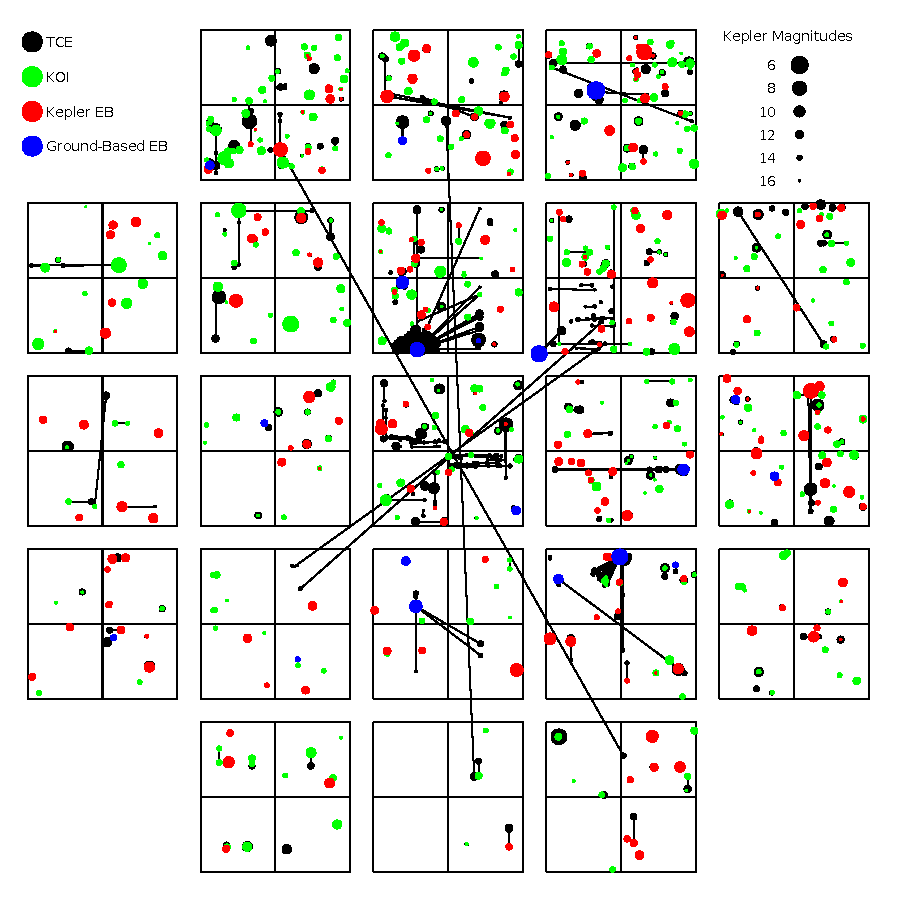
\includegraphics[width=\linewidth]{CCDPlot.pdf}
\caption{Distribution of ephemeris matches on the focal plane. Symbol size scales with magnitude, while color represents the catalog in which the contaminating source was found. Blue indicates that the true transit is from a variable star only known as a result of ground-based observations. Red circles are stars listed in the \kepler{} EBWG catalog, green are KOIs, and black are TCEs. Black lines connect false positive matches with the most likely contaminating parent. In most cases parent and child are so close that the connecting line is invisible.}
\label{ephemmatchfig}
\end{figure*}


% The larger number of matches compared to the Q1--Q12 and Q1--Q16 catalogs is predominately the result of a much larger short-period false positive population compared to Q1--Q16, and an extended baseline compared to Q1--Q12, coupled with matching all TCEs and not just KOIs. In Q1--Q17~DR24 we identify an additional contamination mechanism, which we label ``Common Systematic''. As mentioned in \S\ref{tcesec}, these are over 200 TCEs that are caused by 3 systematic events that are common to all \kepler{} CCDs and happen to be equidistant in time with a spacing of $\sim$459 days. 

% We also identify 119 examples of ``Column Anomaly'', which is a previously identified mechanism where a parent is able to contaminate a child at large distances if they both lie on the same column of a CCD. This mechanism is particularly pernicious because it does not result in a visible centroid offset; the apparent location of the transit signal via the difference images coincides with the target. If the parent is not observed by \kepler{}, then the child could go undetected as a FP due to the column anomaly, as was recently the case for KOI~6705.01 \citep{Gaidos2015}. The large number of examples of column anomaly now available in the Q1--Q17~DR24 catalog reveals the following:

% \begin{itemize}

% \item Despite equally searching for matches in row and column, no instance of ``row-anomaly'' has been found to occur.

% \item The CCDs are read out in the column direction.

% \item In 91.6\% of cases, the child is at a higher row number than the parent, and thus the parent's pixels are read out before the child's. (The remaining 8.4\% of cases may not have the true parent identified, but rather a sibling, as only the most likely parent is listed, and many parents are unobserved by the spacecraft.)

% \item Most cases show the depth of the child increases over time.

% \item The effect appears to exhibit seasonal depth variations in most cases.

% \item The average depth ratio between parent and child is a factor of $\sim$$10^{4}$, and typically the parent and child have similar magnitudes.

% \end{itemize}

% \noindent Combining these details leads to our conjecture that the column anomaly is due to decreasing charge transfer efficiency over time, likely due to cosmic ray impacts. When the CCD is read out, some charge from the parent is left behind due to charge transfer inefficiency. As the child is read out, and its electrons pass through the pixels where the parent was, the child picks up some of the parent's left-behind electrons. Thus, the variable signal from the parent is induced in the child. As more cosmic ray impacts accumulate over time, the amount of charge left behind by the parent increases, resulting in an increase in contamination, and thus an increase in the observed depth of the child. Seasonal variation is seen as the parent and child rotate between 4 CCDs with season, and the amount of degradation varies with CCD. The average depth ratio, along with the delta magnitudes observed, indicate that a charge transfer efficiency of $\sim$99.99\% is consistent with the observed contamination, i.e., a degradation of $\sim$0.01\%. This is well within the range observed on Hubble's Advanced Camera for Surveys and other spaceborne detectors  \citep[see \S3.7 of][and references therein]{Sirianni2005}.




\subsection{Disposition Scores}

A new feature we introduce in this catalog is the disposition score --- a value between 0 and 1 that indicates the confidence in disposition provided by the Robovetter. For PCs, a higher value indicates more confidence in its disposition. For FPs, a higher value indicates less confidence in its disposition. This feature is desirable to calculate accurate occurrence rates, as users can rank the PC and FP populations by their score and weight them appropriately for their statistics.

The disposition score was calculated by wrapping the Robovetter in a Monte Carlo routine. In each of 10,000 iterations the input metrics for the Robovetter are perturbed from their nominal values by drawing from an asymmetric Gaussian distribution centered on the nominal value. In each iteration the robovetter dispositions each TCE given the new values for each metric. The disposition score is simply the fraction of iterations that result in a disposition of PC. For example, if a PC KOI has a few metrics that are near the Robovetter's thresholds, it will frequently have at least one that is perturbed across a threshold. As a result, many of the iterations will produce a false positive and the candidate will have a low score.  Similarly, if a FALSE POSITIVE KOI barely fails a single metric, the score may be near 0.5, indicating that it was deemed a planet candidate in half of the iterations.

To compute the asymmetric sigma values for the Gaussian distribution, we examine the distribution of the robovetter metric for the injected on-target population. We calculate the positive and negative MAD values for each metric as a function of MES and period. These MAD values are then multiplied by a conversion factor of 1.4826 (ADD REF) to put the variability on the same scale as a standard deviation.

NEED TO MENTION AND CLEAN UP FIGURES

TALK ABOUT SCORE DISTRIBUTION HERE, OR LATER ON IN ANALYSIS?

\begin{figure}
\centering
\includegraphics[width=\linewidth]{Metric-StDev-1.pdf}
\caption{A plot of how we calculated errors for the robovetter score.}
\label{score-fig-1}
\end{figure}

\begin{figure}
\centering
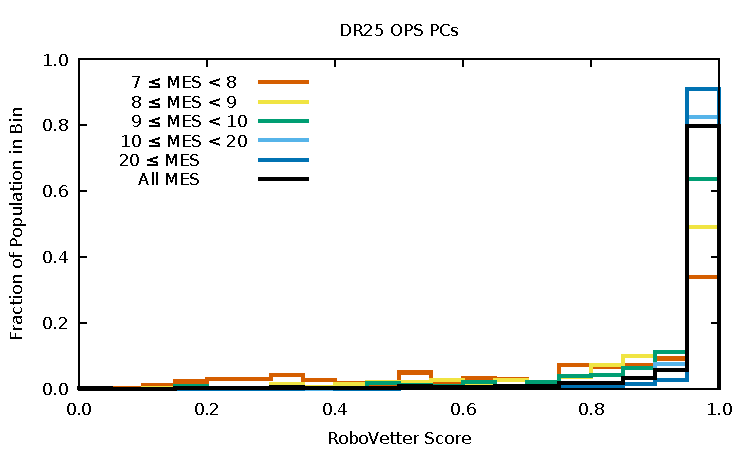
\includegraphics[width=\linewidth]{Scores-1.pdf}
\caption{A plot of how we calculated errors for the robovetter score.}
\label{score-fig-2}
\end{figure}


\subsection{Individual Transit Metrics}

\subsubsection{Marshall -- Individual Transit Shape}
%%Text describing new Marshall algorithm

\citet{Coughlin2016} used the Marshall method \citep{Mullally16} to identify and reject false alarm TCEs caused by short period transients in the data. Marshall fits the proposed transit with models of a transit and various transients and used a Bayesian Information Criterion to decide which model was the best explanation for the data. Simulations in \citet{Mullally16} showed that Marshall was 95\% complete for TCEs with periods $>150$\,days and correctly rejected 66\% of simulated artifact events. The limit on Marshall's effectiveness at eliminating false alarms was it used a parabola to describe the out-of-transit flux, which failed to capture much of the real observed stellar variability. To ensure high completeness, Marshall was tuned to prevent a variable continuum causing true transits to be rejected, at the cost of a lower than ideal effectiveness.

For this catalog, we use a Gaussian Process approach \citep[GP][]{Rasmussen10} to provide an improved continuum model to improve our effectiveness while maintaining our high completeness. Briefly, our approach aims to model the covariance in the lightcurve to better fit the trends in our data.
A similar approach was used by \citet{ForemanMackey16} to model single transits due to very long period planets ($P > 1000$\,days).

Our procedure is as follows. For each individual proposed transit event, we select a snippet of PDC data 30 times the reported transit duration centred on the event. Where the event happens near the start (or end) of a quarter, we take a snippet of similar length anchored at the start (or end) of the quarter. We use the George package \citep{Ambikasaran14} to fit the covariance of the out-of-transit flux with an exponential squared function, $ {\mathrm{Cov(\delta t})} = A \exp{ (\delta t/\ell)^2}$, where $A$ and $\ell$ are tunable parameters. 

We next fit four models to the entire snippet.

\begin{equation}
\left.\begin{aligned}
G(t | A, \ell) + y_0 \\
G(t | A, \ell) + y_0 + S(t)\\
G(t | A, \ell) + y_0 + S(t)(1 - \exp{\beta t})\\
G(t | A, \ell) + y_0 + S(t - \tau/2) - S(t + \tau/2) 
\end{aligned}\right.
\end{equation}

\noindent
where $G$ is the Gaussian Process model with the tunable parameters held fixed to those found earlier, and $y_0$ is a constant offset. $S(t)$ is given by

\begin{equation}
S(t) = \frac{d}{1 - e^{-\gamma (t-t_0)} }
\end{equation}

\noindent
where $d$ and $t_0$ are tunable parameters, while $\gamma$ is held constant. This function, known as a sigmoid (or logistic) function, has a value of 1 for $t<t_0$, 0 for $t>t_0$, and transitions quickly, but smoothly, between the two states. By using a sigmoid and avoiding the discontinuities in present in the models used by the original Marshall algorithm we can use the L-BFGS-B algorithm \citep{Byrd95} available in the Scipy package \footnote{\url{www.scipy.org}} instead of the less robust Neldar-Mead.

The second function models a discrete jump in the data. We fit this model seeded with a negative-going dip at the predicted time of ingress, and also with a positive-going spike at the predicted egress, as we see both features in \Kepler\ data. The third model fits a Sudden Pixel Sensitivity Drop (SPSD) event, probably caused by a cosmic ray hit on the detection. The last model approximates a box transit. By varying the parameter $\gamma$ we could in principle model transit ingress and egress, but find that extra degree of freedom is not necessary to explain the low signal-to-noise events of most concern.

For each transit the Marshall method returns the BIC score, the preferred model and the difference between the preferred model and the sigmoid box fit.  A transit is considered sufficiently bad when the marshall score exceeds a particular threshold, as with the original Marshall algorithm.  However, in a few cases the Gaussian processes fails, yield extremely large, unbelievable BIC values. In these cases the trasit is set to always pass.  Also, for low MES transits, the expected SES of a transit is sufficiently low that Marshall will be unable to distinguish between the ``no transit" model and a low signal-to-noise transit.  Because of this the robovetter uses the following logic when deciding whether a specific transit is not valid :
\begin{equation}

\end{equation}

{\bf Add some kind of discussion of performance}
{\bf Add link to Source Forge code}
 
 
\subsubsection{Skye -- Transits Clustered by Skygroup}

The Skye metric searches for those transit times that have an unusual number of transits at the same time on the same skygroup.   One well known image artifact is called rolling band. \textbf{When two frequencies beat together they create something that is described in the instrument handbook it creates changes in the black level that are both time and spatial dependent.} This effect should cause many transit like events to occur at approximately the same time for all stars on that channel when rolling band occurs. Because the telescope rolls every once each quarter, these rolling band artifact conspire to create TCEs around 370\,d in period.  The Skye metric examines the skyline plot, see Figure\label{f:skyline} for an example, for each skygroup and identifies those times with an excess of transits in a one day bin.  All transits that fall in this bin are marked as an invalid transit.

Skye chooses the threshold for each skygroup with the following logic. For each skygroup the average rate of transits per time bin is found by taking the number of transits associated with TCEs with Periods less than 40?? days. One day bins are created running from 200?? to 1600??, skipping any bin which no transits exist using the entire population of OBS TCEs, this removes time bins for which no data exists for the majority of targets. The average rate of transits per bin (R) is given by the number of transits (N) divided by the number of bins (B) and the scatter in that average would likely be governed by Poisson statistics. We define a threshold as $R + S \times \sqrt{R}$ where S is an arbitrary value that is held constant for all skygroups. Since some transits are known to be clustered, these transits will not contribute evenly to all the bins and create a high value for R. To adjust for this we iteratively remove the transits in bins that are above the threshold and then recalculate R using the new values for both the remaining number of transits and the remaining number of bins. We stop iterating when there are no more peaks and the values converge.

\section{Completeness and Reliability}

\subsection{Catalog Completeness}
\subsubsection{Evaluate recovery of Pixel-level Injected Transits}
\subsubsection{Evaluate recovery of previous KOIs and Confirmed Planets}
\subsubsection{Completeness in Period and MES}

\subsection{Catalog Effectiveness at removing False Positives}
We need a catalog highly effective at removing false positives and false alarms in order to have highly reliable PCs.
\subsubsection{Centroid Robovetter Results for astrophysical FPs}
\subsubsection{Inversion to evaluate Effectiveness for False Alarm removal}
\subsubsection{Evaluate the PC rate of certified FPs}
\subsection{Reliability}


\section{Putting together the KOI Catalog}

The robovetter vets all TCEs, but we only report those that we consider to be transit-like to the KOI table. We must federate our current list with those KOIs we have made before.
\subsection{Federating to known KOIs}
\label{koisec}

\subsection{Model Fits using MCMC}
\label{s:transitfits}

\subsubsection{Comparison between }
\subsection{Deliverables}
We deliver all of the metrics etc..

\section{Overview of the DR25 KOI Catalog}
\subsection{The physical parameters of the planets}
\subsection{New Multi-planet systems}
\subsection{Potentially Rocky Planets in the Habitable Zone}
This is a closer look at some of our most interesting objects.
\subsection{Obvious Problems}

\section{Using This Catalog for Occurrence Rate Calculations}
\subsection{State what the project is providing to make this possible.}


\section{Conclusions}

\acknowledgments
Thanks to GNU parallel \citep{Tange2011a}.

\appendix
\section{List of Acronyms}

\section{Robovetter Minor Flags}
%\section{Robovetter Mnemonic Flags}
\label{minorflagsec}
\red{This needs to be updated with DR25 mnemonic flags.}
In Table~\ref{robodispstab} we list mnemonic flags that describe the results of individual robovetter tests in the comments column. Here we describe the meaning of each flag.

\begin{itemize}
\item[] \textbf{ALT\_ROBO\_ODD\_EVEN\_TEST\_FAIL}: The TCE failed the robovetter's odd-even depth test on the alternate detrending, and thus is marked as a FP due to a significant secondary.
\item[] \textbf{ALT\_SEC\_COULD\_BE\_DUE\_TO\_PLANET}: A significant secondary eclipse was detected in the alternate detrending, but it was determined to possibly be due to planetary reflection and/or thermal emission. While the significant secondary major flag remains set, the TCE is dispositioned as a PC.
\item[] \textbf{ALT\_SEC\_SAME\_DEPTH\_AS\_PRI\_COULD\_BE\_TWICE\_TRUE\_PERIOD}: A significant secondary eclipse was detected in the alternate detrending, but it was determined to be the same depth as the primary within the uncertainties. Thus, the TCE is possibly a PC that was detected at twice the true orbital period. When this flag is set, it acts as an override to other flags such that the significant secondary major flag is not set, and thus the TCE is dispositioned as a PC if no other major flags are set.
\item[] \textbf{ALT\_SIG\_PRI\_MINUS\_SIG\_POS\_TOO\_LOW}: The difference of the primary and positive event significances, computed by the model-shift test using the alternate detrending, is below the threshold $\sigma'_{\rm FA}$. This indicates the primary event is not unique in the phased light curve, and thus the TCE is dispositioned as a FP with the not transit-like major flag set.
\item[] \textbf{ALT\_SIG\_PRI\_MINUS\_SIG\_TER\_TOO\_LOW}: The difference of the primary and tertiary event significances, computed by the model-shift test using the alternate detrending, is below the threshold $\sigma'_{\rm FA}$. This indicates the primary event is not unique in the phased light curve, and thus the TCE is dispositioned as a FP with the not transit-like major flag set.
\item[] \textbf{ALT\_SIG\_PRI\_OVER\_FRED\_TOO\_LOW}: The significance of the primary event divided by the ratio of red noise to white noise in the light curve, computed by the model-shift test using the alternate detrending, is below the threshold $\sigma_{\rm FA}$. This indicates the primary event is not significant compared to the amount of systematic noise in the light curve, and thus the TCE is dispositioned as a FP with the not transit-like major flag set.
\item[] \textbf{CENTROID\_SIGNIF\_UNCERTAIN}: The significance of the centroid offset cannot be measured to high enough precision, and thus the centroid module can not confidently disposition the TCE as a FP. This is typically due to having only a very small number (3 or 4) of offset measurements, all with low SNR.
\item[] \textbf{CLEAR\_APO}: The TCE was marked as a FP due to a centroid offset because the transit occurs on a star that is spatially resolved from the target.
\item[] \textbf{CROWDED\_DIFF}: More than one potential stellar image was found in the difference image. The EYEBALL flag is always set when the CROWDED\_DIFF flag is set.
\item[] \textbf{DV\_ROBO\_ODD\_EVEN\_TEST\_FAIL}: The TCE failed the robovetter's odd-even depth test on the DV detrending, and thus is marked as a FP due to a significant secondary.
\item[] \textbf{DV\_SEC\_COULD\_BE\_DUE\_TO\_PLANET}: A significant secondary eclipse was detected in the DV detrending, but it was determined to possibly be due to planetary reflection and/or thermal emission. While the significant secondary major flag remains set, the TCE is dispositioned as a PC.  
\item[] \textbf{DV\_SEC\_SAME\_DEPTH\_AS\_PRI\_COULD\_BE\_TWICE\_TRUE\_PERIOD}: A significant secondary eclipse was detected in the DV detrending, but it was determined to be the same depth as the primary within the uncertainties. Thus, the TCE is possibly a PC that was detected at twice the true orbital period. When this flag is set, it acts as an override to other flags such that the significant secondary major flag is not set, and thus the TCE is dispositioned as a PC if no other major flags are set.
\item[] \textbf{DV\_SIG\_PRI\_MINUS\_SIG\_POS\_TOO\_LOW}: The difference of the primary and positive event significances, computed by the model-shift test using the DV detrending, is below the threshold $\sigma'_{\rm FA}$. This indicates the primary event is not unique in the phased light curve, and thus the TCE is dispositioned as a FP with the not transit-like major flag set.
\item[] \textbf{DV\_SIG\_PRI\_MINUS\_SIG\_TER\_TOO\_LOW}: The difference of the primary and tertiary event significances, computed by the model-shift test using the DV detrending, is below the threshold $\sigma'_{\rm FA}$. This indicates the primary event is not unique in the phased light curve, and thus the TCE is dispositioned as a FP with the not transit-like major flag set.  
\item[] \textbf{DV\_SIG\_PRI\_OVER\_FRED\_TOO\_LOW}: The significance of the primary event divided by the ratio of red noise to white noise in the light curve, computed by the model-shift test using the DV detrending, is below the threshold $\sigma_{\rm FA}$. This indicates the primary event is not significant compared to the amount of systematic noise in the light curve, and thus the TCE is dispositioned as a FP with the not transit-like major flag set.  
\item[] \textbf{EYEBALL}: The metrics used by the centroid module are very close to the decision boundaries, and thus the centroid disposition of this TCE is uncertain and warrants further scrutiny. No TCEs are marked as a FP due to a centroid offset if this flag is set.
\item[] \textbf{FIT\_FAILED}: The transit was not fit by a model in DV and thus no difference images were created for use by the centroid module. Thus, the TCE is not failed due to a centroid offset by default. This flag is typically set for very deep transits due to eclipsing binaries.
\item[] \textbf{INVERT\_DIFF}: One or more difference images were inverted, meaning the difference image claims the star got brighter during transit. This is usually due to variability of the target star and suggests the difference image should not be trusted. When this flag is set, the TCE is marked as a candidate that requires further scrutiny, i.e., the EYEBALL flag is set and the TCE is not marked as a FP due to a centroid offset.
\item[] \textbf{KIC\_OFFSET}: The centroid module measured the offset distance relative to the star's recorded position in the Kepler Input Catalog (KIC), not the out of transit centroid. The KIC position is less accurate in sparse fields, but more accurate in crowded fields. If this is the only flag set, there is no reason to believe a statistically significant centroid shift is present \citep{Mullally2015c}.
\item[] \textbf{LPP\_ALT\_TOO\_HIGH}: The LPP value \citep{Thompson2015b}, as computed using the alternate detrending, is above the robovetter threshold. This indicates the TCE is not transit-shaped, and thus is dispositioned as a FP with the not transit-like major flag set.
\item[] \textbf{LPP\_DV\_TOO\_HIGH}: The LPP value, as computed using the DV detrending, is above the robovetter threshold. This indicates the TCE is not transit-shaped, and thus is dispositioned as a FP with the not transit-like major flag set.  
\item[] \textbf{MARSHALL\_FAIL}: The TCE failed the Marshall metric \citep{Mullally2015b}, which indicates that the TCE's individual transits are not transit-shaped and more likely due to instrumental artifacts. Thus, the TCE is dispositioned as a FP with the not transit-like major flag set.
\item[] \textbf{OTHER\_TCE\_AT\_SAME\_PERIOD\_DIFF\_EPOCH}: Another TCE on the same target with a higher planet number was found to have the same period as the current TCE, but a significantly different epoch. This indicates the current TCE is an eclipsing binary with the other TCE representing the secondary eclipse. If the ALT\_SEC\_COULD\_BE\_DUE\_TO\_PLANET and DV\_SEC\_COULD\_BE\_DUE\_TO\_PLANET flags are not set, the TCE is dispositioned as a FP with the significant secondary major flag set.
\item[] \textbf{PARENT\_IS\_X}: The TCE has been identified as a FP due to an ephemeris match. This flag indicates the most likely parent, or true physical source of the signal, where X will be substituted for the parent's name. Note that X is not guaranteed to be the true parent, but simply is the most likely source given the information available.
\item[] \textbf{PERIOD\_ALIAS\_IN\_ALT\_DATA\_SEEN\_AT\_X:1}: Using the results of the model-shift test (specifically the phases of the primary, secondary, and tertiary events) a possible period alias is seen at X:1, where X is an integer. This indicates the TCE has likely been detected at a period that is X times longer than the true orbital period. This flag is currently informational only and not used to declare any TCE a FP.
\item[] \textbf{RESID\_OF\_PREV\_TCE}: The TCE has the same period and epoch as a previous transit-like TCE. This indicates the current TCE is simply a residual artifact of the previous TCE after it was removed from the light curve. Thus, the current TCE is dispositioned as a FP with the not transit-like major flag set.
\item[] \textbf{SAME\_P\_AS\_PREV\_NTL\_TCE}: The current TCE has the same period as a previous TCE that was dispositioned as FP with the not transit-like major flag set. This indicates that the current TCE is due to the same not transit-like signal. Thus, the current TCE is dispositioned as a FP with the not transit-like major flag set.
\item[] \textbf{SATURATED}: The star is saturated. The assumptions employed by the centroid robovetter module break down for saturated stars, so the TCE is marked as a candidate requiring further scrutiny, i.e., the EYEBALL flag is set and the TCE is not marked as a FP due to a centroid offset.
\item[] \textbf{SEASONAL\_DEPTH\_DIFFS\_IN\_ALT}: There appears to be a significant difference in the computed TCE depth when using the alternate detrending light curves from different seasons. This indicates significant light contamination is present, usually due to a bright star at the edge of the image, which may or may not be the source of the signal. As it is impossible to determine whether or not the TCE is on-target from this flag alone, it is currently informational only and not used to declare any TCE a FP.
\item[] \textbf{SEASONAL\_DEPTH\_DIFFS\_IN\_DV}: There appears to be a significant difference in the computed TCE depth when using the DV detrending light curves from different seasons. This indicates significant light contamination is present, usually due to a bright star at the edge of the image, which may or may not be the source of the signal. As it is impossible to determine whether or not the TCE is on-target from this flag alone, it is currently informational only and not used to declare any TCE a FP.  
\item[] \textbf{SIG\_SEC\_IN\_ALT\_MODEL\_SHIFT}: The significance of the secondary event divided by the ratio of red noise to white noise in the light curve, computed by the model-shift test using the alternate detrending, is above the threshold $\sigma_{\rm FA}$. Also, the difference between the secondary and tertiary event significances, and the difference between the secondary and positive event significances, both computed by the model-shift test using the alternate detrending, is above the threshold $\sigma'_{\rm FA}$. This indicates that there is a unique and significant secondary event in the light curve, i.e., a secondary eclipse. Thus, assuming the ALT\_SEC\_COULD\_BE\_DUE\_TO\_PLANET flag is not set, the TCE is dispositioned as a FP with the significant secondary flag set.
\item[] \textbf{SIG\_SEC\_IN\_DV\_MODEL\_SHIFT}: The significance of the secondary event divided by the ratio of red noise to white noise in the light curve, computed by the model-shift test using the DV detrending, is above the threshold $\sigma_{\rm FA}$. Also, the difference between the secondary and tertiary event significances, and the difference between the secondary and positive event significances, both computed by the model-shift test using the DV detrending, is above the threshold $\sigma'_{\rm FA}$. This indicates that there is a unique and significant secondary event in the light curve, i.e., a secondary eclipse. Thus, assuming the DV\_SEC\_COULD\_BE\_DUE\_TO\_PLANET flag is not set, the TCE is dispositioned as a FP with the significant secondary flag set.
\item[] \textbf{SIGNIF\_OFFSET}: There is a statistically significant shift in the centroid during transit. This indicates the variability is not due to the target star. Thus, the TCE is dispositioned as a FP with the centroid offset major flag set.
\item[] \textbf{THIS\_TCE\_IS\_A\_SEC}: The TCE is determined to have the same period, but different epoch, as a previous transit-like TCE. This indicates that the current TCE corresponds to the secondary eclipse of an eclipsing binary (or planet if the ALT\_SEC\_COULD\_BE\_DUE\_TO\_PLANET or DV\_SEC\_COULD\_BE\_DUE\_TO\_PLANET flags are set.) Thus, the current TCE is dispositioned as a FP with both the not transit-like and significant secondary major flags set.
\item[] \textbf{TOO\_FEW\_CENTROIDS}: The PRF centroid fit used by the centroid module does not always converge, even in high SNR difference images. This flag is set if centroid offsets are recorded for fewer than 3 high SNR difference images.
\item[] \textbf{TOO\_FEW\_QUARTERS}: Fewer than 3 difference images of sufficiently high SNR are available, and thus very few tests in the centroid module are applicable to the TCE. If this flag is set in conjunction with the CLEAR\_APO flag, the source of the transit may be on a star clearly resolved from the target.
\item[] \textbf{TRANSITS\_NOT\_CONSISTENT}: The TCE had a max\_ses\_in\_mes / mes ratio of greater than 0.9, and a period greater than 90 days. This indicates that the TCE is dominated by a single large event, and thus is due to a systematic feature such as a sudden pixel sensitivity dropout. Thus, the TCE is dispositioned as a FP with the not transit-like major flag set.
\end{itemize}

\bibliographystyle{aasjournal}
\bibliography{References.bib}

\end{document}


%\subsection{Individual Metrics, updates and improvements}

%\paragraph{Not-Transit-Like Metrics} 
%Some metrics that determine if a TCE is not-transit-like operate on the individual transits. We define not-transit-like as anything that does not have three periodic, box- or v-shaped events. Primarily we try to eliminate TCEs caused by instrumental or data-reduction-pipeline effects (like Sudden Pixel Sensitivity Drop Outs or detrending artifacts) and smoothly varying variable stars (pulsators, contact binaries and ellipsoidal binaries) with this high level flag.   These individual metrics are as follows: Marshall, Skye, Chases, and Rubble. The Robovetter also recalculates the MES based on the good transits and counts the number of good transits to decide which TCEs should be considered False Positives. 

%
\subsection{Individual Transit Metrics}

\subsubsection{Marshall -- Individual Transit Shape}
%%Text describing new Marshall algorithm

\citet{Coughlin2016} used the Marshall method \citep{Mullally16} to identify and reject false alarm TCEs caused by short period transients in the data. Marshall fits the proposed transit with models of a transit and various transients and used a Bayesian Information Criterion to decide which model was the best explanation for the data. Simulations in \citet{Mullally16} showed that Marshall was 95\% complete for TCEs with periods $>150$\,days and correctly rejected 66\% of simulated artifact events. The limit on Marshall's effectiveness at eliminating false alarms was it used a parabola to describe the out-of-transit flux, which failed to capture much of the real observed stellar variability. To ensure high completeness, Marshall was tuned to prevent a variable continuum causing true transits to be rejected, at the cost of a lower than ideal effectiveness.

For this catalog, we use a Gaussian Process approach \citep[GP][]{Rasmussen10} to provide an improved continuum model to improve our effectiveness while maintaining our high completeness. Briefly, our approach aims to model the covariance in the lightcurve to better fit the trends in our data.
A similar approach was used by \citet{ForemanMackey16} to model single transits due to very long period planets ($P > 1000$\,days).

Our procedure is as follows. For each individual proposed transit event, we select a snippet of PDC data 30 times the reported transit duration centred on the event. Where the event happens near the start (or end) of a quarter, we take a snippet of similar length anchored at the start (or end) of the quarter. We use the George package \citep{Ambikasaran14} to fit the covariance of the out-of-transit flux with an exponential squared function, $ {\mathrm{Cov(\delta t})} = A \exp{ (\delta t/\ell)^2}$, where $A$ and $\ell$ are tunable parameters. 

We next fit four models to the entire snippet.

\begin{equation}
\left.\begin{aligned}
G(t | A, \ell) + y_0 \\
G(t | A, \ell) + y_0 + S(t)\\
G(t | A, \ell) + y_0 + S(t)(1 - \exp{\beta t})\\
G(t | A, \ell) + y_0 + S(t - \tau/2) - S(t + \tau/2) 
\end{aligned}\right.
\end{equation}

\noindent
where $G$ is the Gaussian Process model with the tunable parameters held fixed to those found earlier, and $y_0$ is a constant offset. $S(t)$ is given by

\begin{equation}
S(t) = \frac{d}{1 - e^{-\gamma (t-t_0)} }
\end{equation}

\noindent
where $d$ and $t_0$ are tunable parameters, while $\gamma$ is held constant. This function, known as a sigmoid (or logistic) function, has a value of 1 for $t<t_0$, 0 for $t>t_0$, and transitions quickly, but smoothly, between the two states. By using a sigmoid and avoiding the discontinuities in present in the models used by the original Marshall algorithm we can use the L-BFGS-B algorithm \citep{Byrd95} available in the Scipy package \footnote{\url{www.scipy.org}} instead of the less robust Neldar-Mead.

The second function models a discrete jump in the data. We fit this model seeded with a negative-going dip at the predicted time of ingress, and also with a positive-going spike at the predicted egress, as we see both features in \Kepler\ data. The third model fits a Sudden Pixel Sensitivity Drop (SPSD) event, probably caused by a cosmic ray hit on the detection. The last model approximates a box transit. By varying the parameter $\gamma$ we could in principle model transit ingress and egress, but find that extra degree of freedom is not necessary to explain the low signal-to-noise events of most concern.

For each transit the Marshall method returns the BIC score, the preferred model and the difference between the preferred model and the sigmoid box fit.  A transit is considered sufficiently bad when the marshall score exceeds a particular threshold, as with the original Marshall algorithm.  However, in a few cases the Gaussian processes fails, yield extremely large, unbelievable BIC values. In these cases the trasit is set to always pass.  Also, for low MES transits, the expected SES of a transit is sufficiently low that Marshall will be unable to distinguish between the ``no transit" model and a low signal-to-noise transit.  Because of this the robovetter uses the following logic when deciding whether a specific transit is not valid :
\begin{equation}

\end{equation}

{\bf Add some kind of discussion of performance}
{\bf Add link to Source Forge code}
 
 
\subsubsection{Skye -- Transits Clustered by Skygroup}

The Skye metric searches for those transit times that have an unusual number of transits at the same time on the same skygroup.   One well known image artifact is called rolling band. \textbf{When two frequencies beat together they create something that is described in the instrument handbook it creates changes in the black level that are both time and spatial dependent.} This effect should cause many transit like events to occur at approximately the same time for all stars on that channel when rolling band occurs. Because the telescope rolls every once each quarter, these rolling band artifact conspire to create TCEs around 370\,d in period.  The Skye metric examines the skyline plot, see Figure\label{f:skyline} for an example, for each skygroup and identifies those times with an excess of transits in a one day bin.  All transits that fall in this bin are marked as an invalid transit.

Skye chooses the threshold for each skygroup with the following logic.  For each skygroup the average rate of transits per time bin is found by taking the number of transits associated with TCEs with Periods less than 40?? days. One day bins are created running from 200?? to 1600??, skipping any bin which no transits exist using the entire population of OBS TCEs, this removes time bins for which no data exists for the majority of targets.  The average rate of transits per bin (R) is given by the number of transits (N) divided by the number of bins (B) and the scatter in that average would likely be governed by Poisson statistics.  We define a threshold as $R + S \times \sqrt{R}$ where S is an arbitrary value that is held constant for all skygroups.  Since some transits are known to be clustered, these transits will not contribute evenly to all the bins and create a high value for R. To adjust for this we iteratively remove the transits in bins that are above the threshold and then recalculate R using the new values for both the remaining number of transits and the remaining number of bins. We stop iterating when there are no more peaks and the values converge.

\subsubsection{Chases -- Asymmetric SES}

\subsubsection{Rubble -- Transits with little data}




%\begin{enumerate}
%\item Marshall
%%%Text describing new Marshall algorithm

\citet{Coughlin2016} used the Marshall method \citep{Mullally16} to identify and reject false alarm TCEs caused by short period transients in the data. Marshall fits the proposed transit with models of a transit and various transients and used a Bayesian Information Criterion to decide which model was the best explanation for the data. Simulations in \citet{Mullally16} showed that Marshall was 95\% complete for TCEs with periods $>150$\,days and correctly rejected 66\% of simulated artifact events. The limit on Marshall's effectiveness at eliminating false alarms was it used a parabola to describe the out-of-transit flux, which failed to capture much of the real observed stellar variability. To ensure high completeness, Marshall was tuned to prevent a variable continuum causing true transits to be rejected, at the cost of a lower than ideal effectiveness.

For this catalog, we use a Gaussian Process approach \citep[GP][]{Rasmussen10} to provide an improved continuum model to improve our effectiveness while maintaining our high completeness. Briefly, our approach aims to model the covariance in the lightcurve to better fit the trends in our data.
A similar approach was used by \citet{ForemanMackey16} to model single transits due to very long period planets ($P > 1000$\,days).

Our procedure is as follows. For each individual proposed transit event, we select a snippet of PDC data 30 times the reported transit duration centred on the event. Where the event happens near the start (or end) of a quarter, we take a snippet of similar length anchored at the start (or end) of the quarter. We use the George package \citep{Ambikasaran14} to fit the covariance of the out-of-transit flux with an exponential squared function, $ {\mathrm{Cov(\delta t})} = A \exp{ (\delta t/\ell)^2}$, where $A$ and $\ell$ are tunable parameters. 

We next fit four models to the entire snippet.

\begin{equation}
\left.\begin{aligned}
G(t | A, \ell) + y_0 \\
G(t | A, \ell) + y_0 + S(t)\\
G(t | A, \ell) + y_0 + S(t)(1 - \exp{\beta t})\\
G(t | A, \ell) + y_0 + S(t - \tau/2) - S(t + \tau/2) 
\end{aligned}\right.
\end{equation}

\noindent
where $G$ is the Gaussian Process model with the tunable parameters held fixed to those found earlier, and $y_0$ is a constant offset. $S(t)$ is given by

\begin{equation}
S(t) = \frac{d}{1 - e^{-\gamma (t-t_0)} }
\end{equation}

\noindent
where $d$ and $t_0$ are tunable parameters, while $\gamma$ is held constant. This function, known as a sigmoid (or logistic) function, has a value of 1 for $t<t_0$, 0 for $t>t_0$, and transitions quickly, but smoothly, between the two states. By using a sigmoid and avoiding the discontinuities in present in the models used by the original Marshall algorithm we can use the L-BFGS-B algorithm \citep{Byrd95} available in the Scipy package \footnote{\url{www.scipy.org}} instead of the less robust Neldar-Mead.

The second function models a discrete jump in the data. We fit this model seeded with a negative-going dip at the predicted time of ingress, and also with a positive-going spike at the predicted egress, as we see both features in \Kepler\ data. The third model fits a Sudden Pixel Sensitivity Drop (SPSD) event, probably caused by a cosmic ray hit on the detection. The last model approximates a box transit. By varying the parameter $\gamma$ we could in principle model transit ingress and egress, but find that extra degree of freedom is not necessary to explain the low signal-to-noise events of most concern.


{\bf Add some kind of discussion of performance}

%\item Skye
%\item ChASES
%\item Rubble
%\item Rocky
%\item Grouping single transit failures and recalculating MES and counting the number of transits.
%\end{enumerate}

%Other metrics operate on data gathered using all the photometric data to determine if the transit signal is transit-like.  These metrics are as follows:

%\begin{enumerate}
%\item LPP retrained
%\item Model Shift Uniqueness
%\item SWEET -- for N flag
%\item Grouped ChASES
%\item Model Shift DMM
%\item Model Shift Shape Metric
%\item MES/SES

%\end{enumerate}

%\paragraph{Significant Secondary Metrics}
%Some metrics look for evidence that a transit-like signal is actually due to %an eclipsing binary (foreground or background).  It primarily looks for %evidence of a secondary eclipse, but there are also metrics to look for %ellipsoidal

%\begin{enumerate}
%\item Model Shift Secondary
%\item Model Shift Odd-Even
%\item Simple Odd-Even
%\item SWEET -- for S flag (we might need to combine N and S for this reason)
%\end{enumerate}


%\paragraph{Centroid Offset} We vet the catalog for evidence that the the target is a false positive because of a background eclipsing binary. The Centroid Robovetter us run on the pixel level data to determine if this is the case.  This is unchanged from the previous two catalogs.  The \textbf{Ghostbuster metric} is also used to determine if the TCE signal is from pixels other than the star.

%\paragraph{Ephemeris Matching} We also look for evidence that 
